% !TeX spellcheck = pt_BR
\RequirePackage[l2tabu, orthodox]{nag}
%Avisa se houver pacotes antigos ou problemas comuns. Tem de se usar antes do documentclass


\documentclass[a4paper,twocolumn,final,11pt]{article}
%Mudar entre "draft" e "final" para fazer o documento rascunho/final
\setlength{\columnsep}{0.8cm}
%\setlength{\parskip}{.05em}

%Pacote hyperref ---------------
%\usepackage{hyperref}
%Cria hiperligacoes dentro do documento para saltar entre partes; ha muitas interferencias com outros pacotes e pode dar problemas

%Pacotes para LaTeX -------------
\begingroup\expandafter\expandafter\expandafter\endgroup
\expandafter\ifx\csname IncludeInRelease\endcsname\relax
\usepackage{fixltx2e}
\fi
%Resolve problemas comuns

%Aparencia ----------------------
\usepackage[a4paper,top=2.8cm, bottom=3cm, left=1.6cm, right=1.6cm]{geometry}
\usepackage[a4paper]{geometry}
%Acertar aspecto da pagina, como as margens	

\usepackage[stretch=10]{microtype}
%Melhora o espaçamento entre as palavras, reduz a hifenação, formata melhor o bloco de texto.

%Pacotes para Portugues ----------
%\usepackage[utf8]{inputenc}
\usepackage[portuguese]{babel}
\usepackage[latin1]{inputenc}


\usepackage{indentfirst}
%Indenta a primeira linha dos paragrafos

%\usepackage{libertineRoman}

\usepackage{libertine}
\usepackage{lmodern}
\usepackage[T1]{fontenc}
%Tipo de letra vectorial, com melhor qualidade, para usar o T1. Se o tipo de letra aparecer pixelizado, activar este pacote. Para evitar utilizar o lmodern, pode-se instalar o pacote cm-super.

%Tabelas ----------------------
\usepackage{booktabs}
%Tabelas com melhor aparencia

\usepackage{array}
%Melhor controlo e aparencia de colunas

\usepackage{tabularx}
%Dimensionamento automatico de colunas
\usepackage[export]{adjustbox}
\usepackage{caption}

\usepackage{longtable}
%Para criar tabelas longas

%Imagens -----------------------------
\usepackage{graphicx}
%Para introduzir graficos
%definição bonita de infinito
\def\infinity{\rotatebox{90}{8}}
\usepackage[font={small}]{caption}
%Pacote de legendas de imagens/tabelas

\usepackage{subcaption}
%Para por legendas em sub-figuras

%Matematica ------------------
\usepackage{amsmath}
\usepackage{amssymb}
%\usepackage{fixmath}
%Ambiente e simbolos para matematica - necessarios se se usar matematica. O fixmath corrige alguns problemas com o pacote de simbolos.

%\usepackage{amsthm}
%Ambiente para escrever teoremas

\usepackage{mathtools}

\usepackage{nicefrac}
%Permite usar fracções em texto, com o comando \nicefrac[]{}{}

\usepackage{siunitx}
%Permite usar sistemas de unidades e colunas de tabelas alinhadas pelo ponto decimal. Para escrever unidades: \si{m/s}. Para formatar números \num{2.99e6}

\usepackage{blindtext}


%Para por codigo no documento --------------
\usepackage{xcolor}
\definecolor{gray1}{rgb}{0.92,0.92,0.92}
\definecolor{gray2}{rgb}{0.95,0.95,0.95}
\definecolor{gray3}{rgb}{0.5,0.5,0.5}

\usepackage{listings}

%\definecolor{mygreen}{rgb}{0,0.6,0}
\definecolor{commentgreen}{rgb}{.2,0.6,.2}
\definecolor{mygray}{rgb}{0.5,0.5,0.5}
\definecolor{stringmauve}{rgb}{0.58,0,0.82}

\usepackage{inconsolata}
\lstset{
	%keywordstyle=\bfseries
	breaklines=true,
	captionpos=t,
	basicstyle=\footnotesize\ttfamily,
	xleftmargin=.1\textwidth,
	xrightmargin=.1\textwidth,
	framesep=0pt,
	tabsize=4,
	showstringspaces=false,
	numbers=left,
	numberstyle=\scriptsize\ttfamily,
	numbersep=10pt,
	commentstyle=\slshape\color{commentgreen},
	keywordstyle=\bfseries\color{blue},
	stringstyle=\color{stringmauve},
	extendedchars=true,
	literate={á}{{\'a}}1 {ã}{{\~a}}1 {â}{{\^a}}1 {à}{{\`a}}1 {é}{{\'e}}1 {É}{{\'E}}1 {ê}{{\^e}}1 {ê}{{\^e}}1 {Ê}{{\^E}}1 {í}{{\'i}}1 {ó}{{\'o}}1 {õ}{{\~o}}1 {ô}{{\^o}}1 {ú}{{\'u}}1 {ç}{{\c c}}1 {λ}{{$\lambda$}}1 {θ}{{$\theta$}}1 {π}{{$\pi$}}1 {√}{{$\sqrt{}$}}1 {ẋ}{{$\dot{x}$}}1 {ψ}{{$\psi$}}1 {Σ}{{$\Sigma$}}1 {σ}{{$\sigma$}}1, 
}

% Extras ------------------

\setlength{\marginparwidth}{2cm} % problema do todonotes
%para criar notas no documento
\usepackage{todonotes}
\usepackage{epstopdf}  % Para os gráficos do gnuplot funcionarem
\epstopdfsetup{outdir=./}
%\usepackage{enumerate}
\usepackage{enumitem}  % Para personalisar enumerates e itemizes
\usepackage{float}  % Permite usar \begin{figure/table/etc}[H]... para forçar os floats a ficarem no sítio
\usepackage{placeins}  % Para controlar floats
\usepackage{physics}  % Se Jesus fosse um pacote seria este

\usepackage{url}  % Links com \url{}
%\usepackage{makecell}  % Fazer tabelas mais complicadas (usei para estrutura)
%\usepackage{mhchem}  % Reaccoes quimicas


\newcommand{\overbar}[1]{\mkern 1.5mu\overline{\mkern-1.5mu#1\mkern-1.5mu}\mkern 1.5mu}

\usepackage[makeroom]{cancel}  % \cancel{} para cortar termos
\renewcommand{\CancelColor}{\color{gray}}
\usepackage{amsfonts}

\newcommand\numberthis{\addtocounter{equation}{1}\tag{\theequation}}  % \numberthis para numerar equações. Contrário de \nonumber. Muito útil para só botar número no final de um align*

\newcommand{\CPP}{C\nolinebreak\hspace{-.05em}\raisebox{.4ex}{\tiny\bf +}\nolinebreak\hspace{-.05em}\raisebox{.4ex}{\tiny\bf +}}  % \CPP para escrever C++

%\usepackage{blkarray}  % Matrizes por blocos
%\usepackage[misc]{ifsym}  % Um porradão de símbolos extra, todos bonitinhos em METAFONT

\allowdisplaybreaks[3]  % Para o align poder fluir para várias páginas

% Tikz ------------------
\usepackage{tikz}
\usetikzlibrary{automata,arrows,positioning,calc,decorations}



% User ------------------

% Para mudar o estilo das secções, subsecções, rodapés, etc.
%\renewcommand \thesection    {}
%\renewcommand \thesubsection {\arabic{subsection}. }
%\renewcommand \thefootnote   {$\star$}

\newcommand{\eqv}{\Leftrightarrow}  % Atalho para o <=> (\eqv em vez de \Leftrightarrow)
%\renewcommand{\vec}{\vb}  % Mudar o \vec para negrito
%\newcommand{\nome}{definição, pode conter \comandos}  % Para fazer mais atalhos

\let\oldref\ref
\renewcommand{\ref}[1]{(\oldref{#1})}


%usar varias colunas
\usepackage{multicol}
%para mudar o estilo do itemize
\renewcommand\labelitemi{--}
%para colocar imagens ao lado do texto
\usepackage{wrapfig}

\usepackage{multirow}

\usepackage{appendix}
\addto\captionsportuguese{%
	\renewcommand\appendixname{Anexo}
	\renewcommand\appendixpagename{Anexos}
}

% remover o "referencias" do thebibliography
%\usepackage{etoolbox}
%\patchcmd{\thebibliography}{\section*{\refname}}{}{}{}

\usepackage{fancyhdr}
% ---------------------
% ----- Documento -----
% ---------------------
\pagestyle{fancy}
\lhead{Universidade de Coimbra}
\rhead{Faculdade de Ciências e Tecnologia}



\title{
	\includegraphics[width=0.5\textwidth]{FCTUC_H_FundoClaro.eps} \\
	\vspace{0.5cm}
	\bfseries  % para fazer título e subtítulo negrito
	Projecto de robótica médica\\ 
	{\large Controlo e design de trajectória para cirurgias no osso}
}
    \author{Heloisa Barbosa- 2016123252 \\ Rita Monteiro -2016252297}
\date{\today}


\begin{document}



\maketitle

\section{Objectivo}
O objectivo deste trabalho é implementar arquitecturas para o controlo e trajectória de um braço robótico, cujo o intuito é  auxiliar cirurgias no osso. Para o desenvolvimento deste projecto, é necessário ter em consideração a geometria, a cinemática e a dinâmica de modelos de robôs planares.

Implementou-se um robô com 2 links, primeiramente sem um modelo dinâmico e depois com, e de seguida implementou-se  dois controlos de forças ao robô, o de complacência e o de impedância.
Esses controlos são necessários para estudar e aprimorar as interacções possíveis entre o robô e o paciente.
\begin{figure}[H]
	\centering
	\includegraphics[width=0.4\textwidth]{f1.png}
	\caption{Robô planar de 2 links para cirúrgias no osso \cite{project}.}
  \label{fig1}
\end{figure}
Também implementou-se um robô de 3 links. Explorar a redundância do robô através do design de movimento no espaço nulo, permite evitar contacto com órgãos vitais, manter a postura desejada para além da tentativa de maximizar a manipulação do robô.
\begin{figure}[H]
	\centering
	\includegraphics[width=0.4\textwidth]{f2.png}
	\caption{Robô cirúrgico de 3 links \cite{project}.}
  \label{fig2}
\end{figure}


\section{Control Design}
\subsection{ Forward Kinematics}
Considerou-se um robô com 2 links. O modelo geométrico usado é não redundante, o que significa que o espaço de tarefa tem o mesmo grau de liberdade que o espaço das juntas.

As posições angulares são dadas por $q_{1}$ e $q_{2}$. O ângulo $q_{1}$ é referente à origem do referencial e $q_{2}$ refere-se ao ângulo entre o link 1 e o link 2.
De forma a ser possível mapear as posições angulares das juntas ($q$) e em posições X no espaço de tarefa, é estabelecida uma relação entre as mesmas a partir da função \textit{f}: 
\begin{equation}
    X=f(q)
\end{equation}
O espaço de tarefa pode ser descrito como o sistema de coordenadas onde os links se movem para executar uma determinada tarefa.
As coordenadas no espaço de tarefa (X) permitem representar o robô segundo coordenadas cartesianas do \textit{end-effector}. As posições angulares ($q$) permitem saber as variações angulares que o robô sofre.
\begin{equation}
    X=\left[x~y\right]^T
\end{equation}
\begin{equation}
    q=\left[q_{1}~q_{2}\right]^T
\end{equation}

A cinemática do robô é resultado, então, da relação entre as posições do link 1 ($x_1$ e $y_1$) com o ângulo $q_{1}$ e as posições do link 2 ($x_2$ e $y_2$) com os ângulos $q_{1}$ e $q_{2}$.

\begin{equation}
    x_1 = l_1\cos(q_{1})
\end{equation}
\begin{equation}
    y_1 = l_1\sin(q_{1})
\end{equation}
\begin{equation}
    x_2 = x_1 +  l_2\cos(q_{1}+q_{2})
\end{equation}
\begin{equation}
    y_2 = y_1 +  l_2\sin(q_{1}+q_{2})
\end{equation}

Sendo assim, foi implementado no Matlab a função forward\_kinematics:

\begin{equation}
    eixo\_x = p_1\cos(q_{1}) + p_2\cos(q_{1}+q_{2})
\end{equation}
\begin{equation}
    eixo\_y = p_1\sin(q_{1}) + p_2\sin(q_{1}+q_{2})
\end{equation}

$p_1$ e $p_2$ podem ser definidos pelo utilizador, sendo que, por exemplo, caso se pretenda as coordenadas do centro de massa do link 1, igualamos $p_1$  a $lc_1$ e $p_2$  a 0.

\subsection{Jacobiano}
Neste ponto, pretende-se calcular o Jacobiano do \textit{end-effector} e os Jacobianos para cada centro de massa. O Jacobiano é importante porque permite mapear movimentos diferenciais \.{X} no espaço de tarefa em função de movimentos diferenciais ao nível do espaço das juntas.
É possível, então, obter-se a relação entre a velocidade no espaço de tarefa e a velocidade no espaço das juntas: 

\begin{equation}
    \dot{X} = \dot{f}(q)
\end{equation}

Fazendo agora a derivada relativamente às juntas, obtém-se:

\begin{equation}
    \dot{X} = J(q)\dot{q}
\end{equation}

Assim, o Jacobiano do \textit{end-effector} é dado por: 

\begin{equation}
\resizebox{.41\textwidth}{!}{
$Jee=
\begin{bmatrix}
-l_1\sin(q_1) -l_2\sin(q_1+q_2) & -l_2 \sin(q_1+q_2) \\
l_1 \cos(q_1) +l_2 \cos(q_1+q_2) & l_2 \cos(q_1+q_2)
\end{bmatrix}$}
\end{equation}

O Jacobiano para o centro de massa do link 1 é:

\begin{equation}
\resizebox{.2\textwidth}{!}{
$Jvc1=
\begin{bmatrix}
-lc_1 \sin(q_1)  & 0 \\
lc_1 \cos(q_1)  & 0 \\
0 & 0
\end{bmatrix}$}
\end{equation}

Para o centro de massa do link 2, temos:

\begin{equation}
\resizebox{.41\textwidth}{!}{
$Jvc2=
\begin{bmatrix}
-l_1 \sin(q_1)-lc_2 \sin(q_1+q_2)  & -lc_2 \sin(q_1+q_2) \\
 l_1 \cos(q_1)+lc_2 \cos(q_1+q_2) & lc_2 \cos(q_1+q_2)
\end{bmatrix}$}
\end{equation}

Em movimentos angulares, define-se o jacobiano rotacional dado por:
\begin{equation}
Jw1=
\begin{bmatrix}
0 & 0 \\
0 & 0\\
1 & 0
\end{bmatrix}
\end{equation}
e 
\begin{equation}
Jw2=
\begin{bmatrix}
0 & 0 \\
0 & 0\\
1 & 1
\end{bmatrix}
\end{equation}
Os valores iniciais utilizados estão descritos na tabela \ref{initialvalues}.
\begin{table}[H]
	\centering
	\caption{Características do robô}
	\begin{tabular}{@{}cccc@{}}
		\toprule
		$Link$ & Descrição & Notação  & $Valor$ \\
		\midrule
		$1$ & $Massa$ & $m_1$ & $0.4$  \\
		$ $  & $Comprimento$ & $l_1$ & $0.3$ \\
		$ $  & $Centro~de~massa$ & $lc_1$ & $\frac{l_1}{2}$ \\
		$ $  & $Momento~de~$\textit{Inércia} & $I_1$ & $\frac{1}{12} m_1  l_1^{2} $ \\
		$2$ & $Massa$ & $m_2$ & $0.2$   \\	
		$ $ & $Comprimento$ & $l_2$ & $0.15$   \\
		$ $  & $Centro~de~massa$ & $lc_2$ & $\frac{l_2}{2}$ \\
	    $ $  & $Momento~de~$\textit{Inércia} & $I_2$ & $\frac{1}{12} m_2  l_2^{2} $ \\
		\bottomrule
	\end{tabular}
	\label{initialvalues}
\end{table}
\subsection{M(q), C(q,\.{q}), g(q)}
Neste tópico pretende-se obter a dinâmica do robô através da mecânica Lagrangiana. Esta é uma re-formulação das leis de Newton, a qual considera as relações entre energias.
O Lagragiano do robô pode ser descrito como:
\begin{equation}
   L(q.\dot{q})=E(q,\dot{q})-U(q)
   \label{eqLagranRobo}
\end{equation}
Sendo que E(q,\.{q}) é um escalar representando a energia cinética, e U(q) um escalar representando a energia potencial.

A energia cinética é dada pela equação:
\begin{equation}
    E(q,\dot{q})=\frac{1}{2}\dot{q}^{T}M(q)(\dot{q})
\end{equation}
Sendo M(q) a matriz de inércia e dada pela equação:
\begin{equation*}
\resizebox{.5\textwidth}{!}{
$M(q)= \sum_{i=1}^{n} \left[m_iJ_{vi}(q)^TJ_{vi}(q)+_{wi}(q)^TR_i(q)I_iR_i(q)^TJ_{wi}(q)\right]$}
\end{equation*}
A matriz de inércia para o robô é então: 
\begin{equation}
MassNumeric=
\begin{bmatrix}
M_{11} & M_{12} \\
M_{21} & M_{22}
\end{bmatrix}
\end{equation}
Em que os termos da matriz são dados por:
\begin{align*}
    M_{11} = & l_1^{\frac{2}{5}}+\frac{(2\cos(q_2)l_1lc_2)}{5}+m_1lc_1^2+\frac{lc_2^2}{5}+\\
    & \hspace{3.6cm} +I_{1czz}+I_{2czz} \\
    M_{12} = & \frac{lc_2^2}{5}+\frac{l_1\cos(q_2)lc_2}{5} + I_{2czz}\\
    M_{21} = & \frac{lc_2^2}{5} + \frac{l_1\cos(q_2)lc_2}{5}+ I_{2czz}\\
    M_{22} = & \frac{lc_2^2}{5} + I_{2czz}
\end{align*}
A energia potencial é dada por:
\begin{equation}
    U(q)=-g_{c}^Tr_c(q)m_c
\end{equation}
A matriz para a energia potencial é definida como:
\begin{equation}
U\_numeric=
\begin{bmatrix}
U_{11} 
\end{bmatrix}
\end{equation}
Sendo os seus termos dados por:
\begin{align*}
    U_{11} = & -g_2m_2(R_{2y}+lc_2\sin(q_1+q_2))-\\
    &  -g_1m_2(lc_2\cos(q_1+q_2)+lc_1\cos(q_1))\\
    &-g_1lc_1m_c\cos(q_1)-g_2lc_1m_1\sin(q_1)
\end{align*}

O $\tau$ é a generalização do torque que atua em $q$ e é descrito pela equação:
\begin{equation}
   \tau= M(q)\ddot{q}+v(q,\dot{q})+g(q)
   \label{taueq}
\end{equation}
O termo $v(q,\dot{q})$ é o termo de Coriolis, e pode ser descrito na forma: 
\begin{equation}
   v(q,\dot{q})=C(q,\dot{q})\dot{q}= \dot{M}(q)\dot{q}-\frac{\partial E (q,\dot{q})}{\partial q}
\end{equation}
A matriz $C(q,\dot{q})$ é dada por:
\begin{equation}
C(q,\dot{q})=\dot{M}(q)-\frac{1}{2}\dot{q}^T\frac{\partial M(q)}{\partial q}
\end{equation}
Com $\dot{M}(q)$ definido por:
\begin{equation}
  \dot{M}(q) =\frac{\partial M }{\partial q_1}\dot{q_1}+\frac{\partial M }{\partial q_2}\dot{q_2}
\end{equation}
E com $\dot{q}^T\frac{\partial M(q)}{\partial q}$ sendo uma matriz coluna, temos então que:
\begin{equation}
CoriolisNum=
\begin{bmatrix}
C_{11} & C_{12} \\
C_{21} & C_{22}
\end{bmatrix}
\end{equation}
Sendo os seus termos:
\begin{align*}
    C_{11} = & 2(dq_2)(l_1)(lc_2)(m_2)\sin(q_2)\\
    C_{12} = & -(dq_2)(l_1)(lc_2)(m_2)\sin(q_2)\\
    C_{21} = &  (dq_1)(l_1)(lc_2)(m_2)\sin(q_2) -\frac{(dq_2l_1lc_2m_2\sin(q_2))}{2}\\
    C_{22} = & \frac{(dq_1l_1lc_2m_2\sin(q_2))}{2}
\end{align*}

Por último, temos a definição de $g(q)$ definida como:
\begin{equation}
    g(q)=\frac{\partial U(q)}{\partial q}
\end{equation}
A qual é uma matriz definida por:
\begin{equation}
gravity\_numeric=
\begin{bmatrix}
G_{11}  \\
G_{21} 
\end{bmatrix}
\end{equation}
Em que os termos da matriz são dados por:
\begin{align*}
    G_{11} = & g_1m_2(lc_2\sin(q_1 + q_2) + l_1\sin(q_1)) -\\ &-g_2m_2(lc_2\cos(q_1 + q_2) + l_1\cos(q_1)) -\\ &-g_2lc_1m_1\cos(q_1) + g_1lc_1m_1\sin(q_1)\\
    G_{21} = & g_1lc_2m_2\sin(q_1 + q_2) - g_2lc_2m_2\cos(q_1 + q_2)\\
\end{align*}

 
\subsection{Simulação do robô}

Com o estudo completo dos fundamentos da dinâmica do robô foi possível fazer uma primeira simulação simples, começando por aplicar os binários $\tau_c = 0$ e $\tau_e= 0$, e as condições iniciais:

\begin{equation}
    q_0=\left[\frac{\pi}{2}~\frac{\pi}{4}\right]^T
\end{equation}

\begin{equation}
    \dot{q}_0=\left[0~0\right]^T
\end{equation}

O único elemento de controlo é dado por $\tau_c$.
Tendo em conta a equação \ref{taueq} e, sabendo que o torque de controlo, $\tau_c$, e que o torque  relativo a forças externas, $\tau_e$, são nulos o torque total, $\tau$, apenas dirá respeito ao torque devido à fricção, $\tau_f$. No entanto, não existem forças externas aplicadas, logo $\tau_f$=0.
Resolvendo a equação em ordem a $\ddot{q}$, obtém-se:

\begin{equation}
   \ddot{q} = M(q)^{-1} (\tau - C(q,\dot{q}) \dot{q} - g(q)) 
   \label{segDeriq}
\end{equation}

Como o binário resultante de todas as forças cartesiana e externas aplicadas ao robô é nulo, apenas a força da gravidade actua sobre o manipulador. Como seria esperado, o robô parte da sua posição inicial e "cai" até estabilizar. 

\begin{figure}[H]
	\centering
	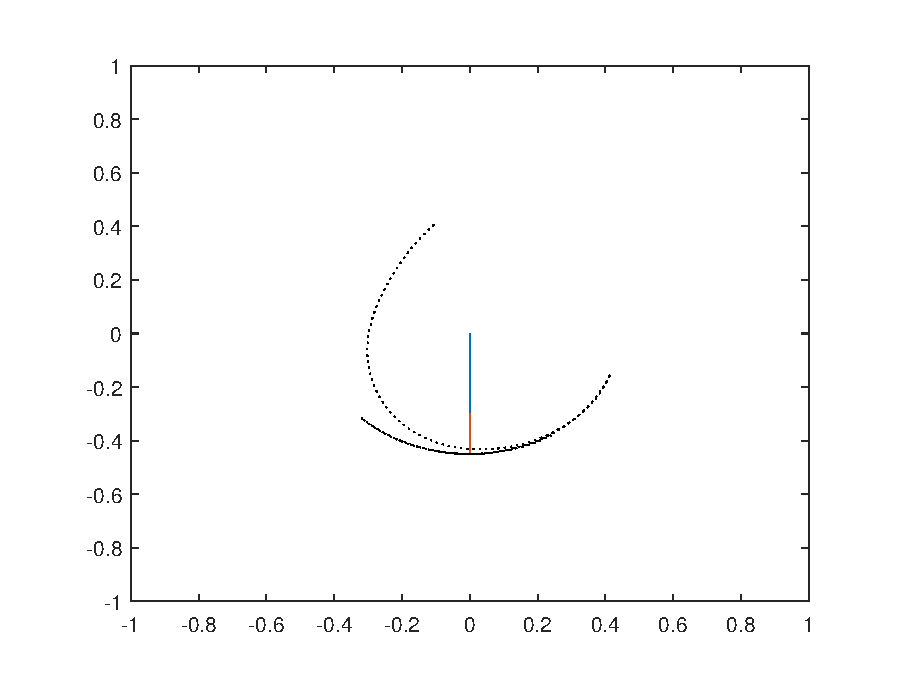
\includegraphics[width=0.4\textwidth]{4.eps}
	\caption{Trajectória do robô quando $\tau_c$=0 e $\tau_f$=0.}
  \label{fig3}
\end{figure}

Fazendo alterações às condições iniciais e ao termo de fricção \textit{Fv}:
\\

Caso 1:

\begin{equation}
    q_0=\left[\frac{\pi}{2}~\frac{\pi}{4}\right]^T
\end{equation}

\begin{equation}
    \dot{q}_0=\left[0~0\right]^T
\end{equation}

\begin{figure}[H]
	\centering
	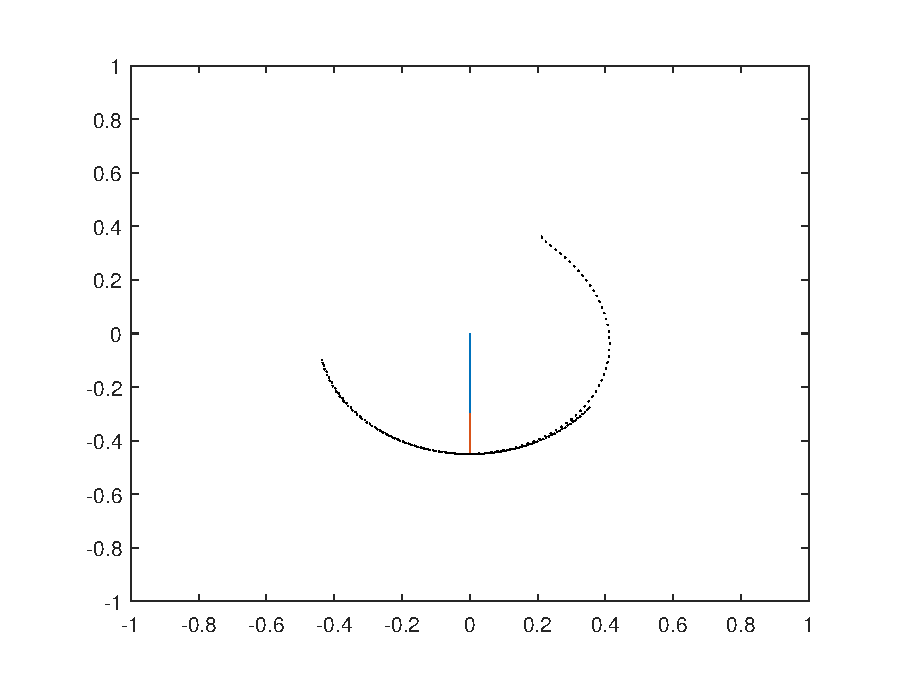
\includegraphics[width=0.4\textwidth]{4_q_pi4_pi4.eps}
	\caption{Trajectória do robô quando $\tau_c$=0 e $\tau_e$=0, e para as condições iniciais do caso 1.}
  \label{fig4}
\end{figure}

No caso 1, o robô tem uma posição inicial diferente, não se observando nenhuma diferença. 
\linebreak

Caso 2:
\begin{equation}
    q_0=\left[\frac{\pi}{4}~\frac{\pi}{4}\right]^T
\end{equation}
\begin{equation}
    \dot{q}_0=\left[\pi~\pi\right]^T
\end{equation}
\begin{figure}[H]
	\centering
	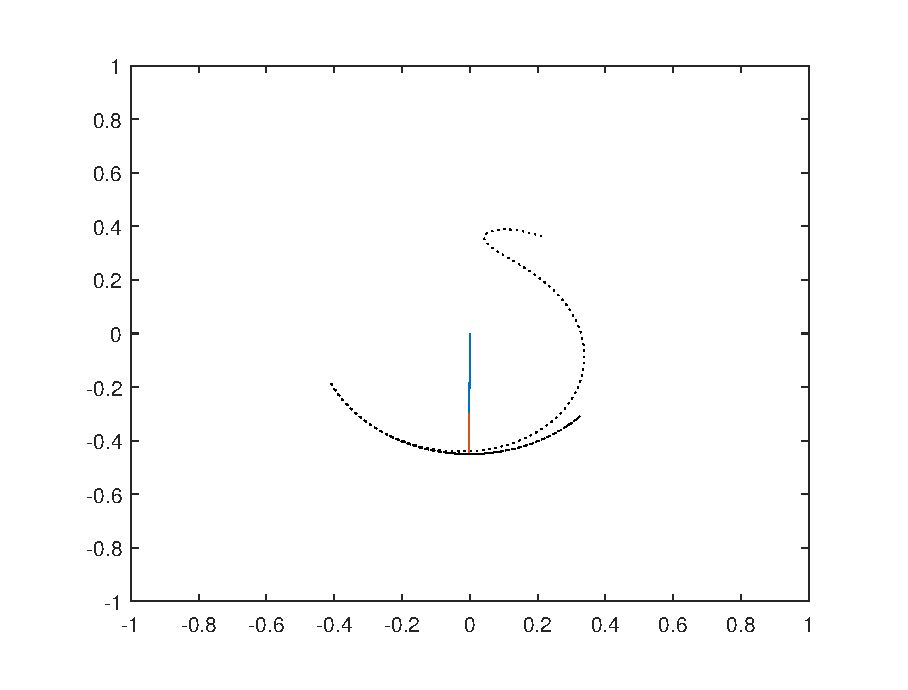
\includegraphics[width=0.4\textwidth]{4_dq_pi_pi.eps}
	\caption{Trajectória do robô quando $\tau_c$=0 e $\tau_e$=0, e para as condições iniciais do caso 2.}
  \label{fig5}
\end{figure}
No caso 2, alterou-se a velocidade inicial das juntas, aumentando de 0 para $\pi$. Isto resultou numa maior velocidade de movimento, assim como numa trajectória com um maior alcance, anterior à estabilização do robô.
\\

Caso 3: 
\begin{equation}
    Fv = 1
\end{equation}
\begin{figure}[H]
	\centering
	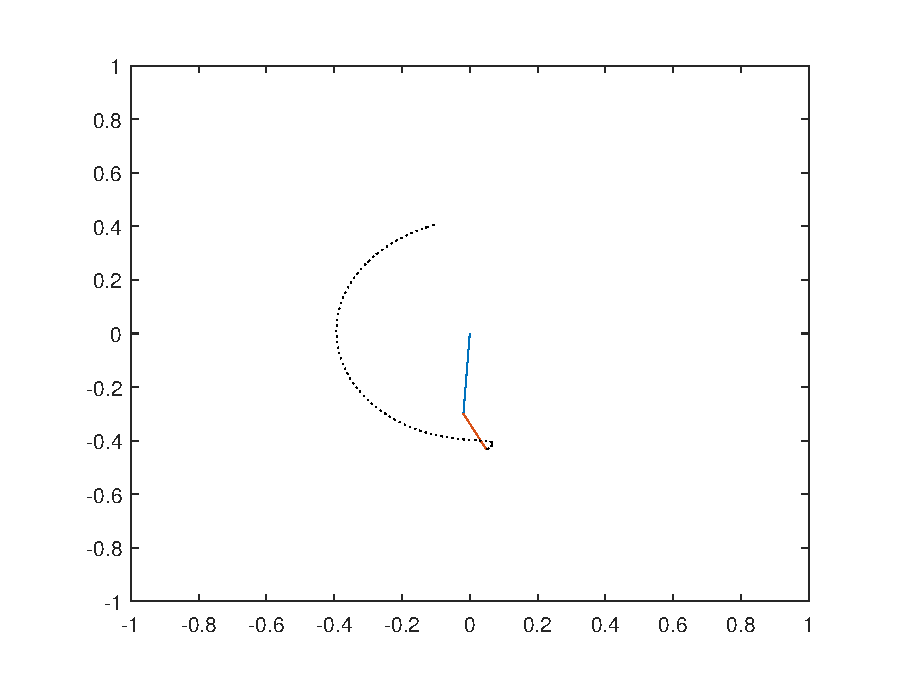
\includegraphics[width=0.4\textwidth]{4_fv_1.eps}
	\caption{Trajectória do robô quando $\tau_c$=0 e $\tau_e$=0, e para \textit{Fv}=1.}
  \label{fig6}
\end{figure}

Caso 4: 
\begin{equation}
    Fv = 0.005
\end{equation}
\begin{figure}[H]
	\centering
	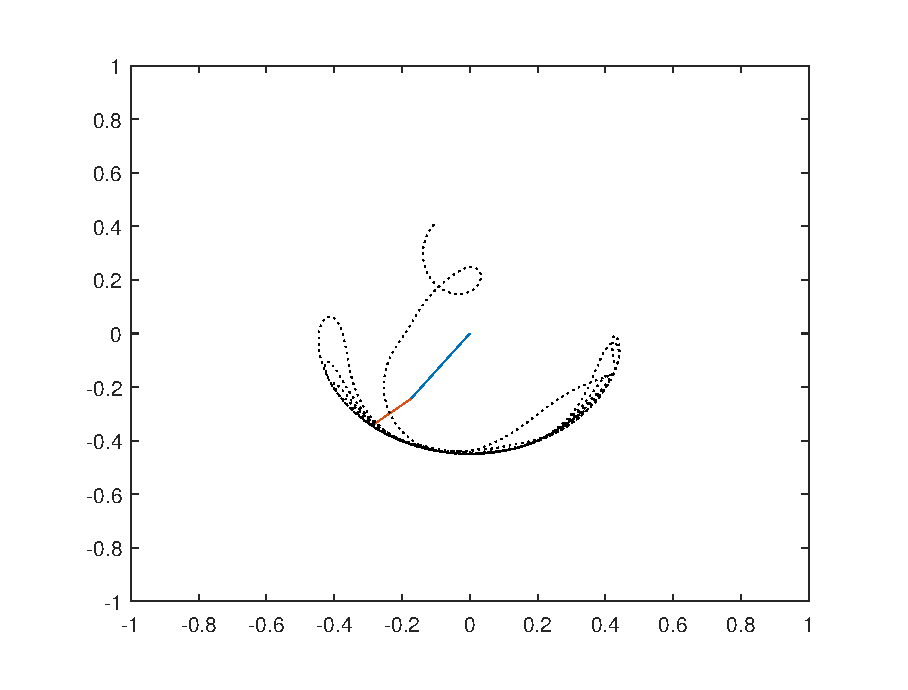
\includegraphics[width=0.4\textwidth]{4_fv_0005.eps}
	\caption{Trajectória do robô quando $\tau_c$=0 e $\tau_e$=0, e para \textit{Fv}=0.005.}
  \label{fig7}
\end{figure}

A partir da observação da trajectória do robô para os casos 3 e 4, percebemos que quanto maior a fricção viscosa, maior é a dissipação de energia durante o movimento e menor será o alcance da trajectória do robô até estabilizar. Se a fricção viscosa for menor, o robô tende a oscilar e a sua trajectória é instável. 

\subsection{Dinâmica do robô com compensação gravítica}

Quando fazemos $\tau$=g(q), estamos a aplicar a compensação da gravidade. A compensação da gravidade equivale a aplicar uma força de intensidade igual mas de sentido oposto à força da gravidade.

\begin{figure}[H]
	\centering
	\includegraphics[width=0.4\textwidth]{5.eps}
	\caption{Trajectória do robô quando $\tau$=g(q).}
  \label{fig8}
\end{figure}

Desta forma, tal como se pode verificar na figura \ref{fig8}, o robô mantém-se parado, isto é, mantém a sua
posição inicial.



\subsection{Aplicação de forças cartesianas ao robô com compensação da gravidade}

A partir deste ponto, inclusive, foi aplicada compensação gravítica nas simulações, garantindo que o movimento do robô apenas se deve ao torque de controlo ou devido a forças externas. Isto seria útil para um caso clínico, uma vez que não seria sentido o peso do braço do robô pelo médico.

Neste ponto, pretende-se estudar a influência de Forças Cartesianas $F_c$ sobre o controlo do movimento, analisando a posição final do robô.

Para controlar o robô, é preciso um binário $\tau_c$ aplicado nas suas juntas. Ao aplicar forças cartesianas, pode-se usar as posições no espaço de tarefa como meio de controlo do robô. 

Assim sendo, em ambiente clínico, o médico estará a aplicar forças cartesianas no \textit{end-effector}, ao longo do seu espaço de trabalho. Estas forças são mapeadas em componentes de $\tau_c$.

Através do Lagrangiano, partindo da equação \ref{eqLagranRobo}, e agora considerando coordenadas cartesianas, obtém-se:

\begin{equation}
    L(X,\dot{X})=E(X,\dot{X})-U(X)
\end{equation}

Também é necessário redefinir a energia cinética E(X,$\dot{X}$) e a energia potencial U(X) do sistema: 

\begin{equation}
    E(X,\dot{X})=\frac{1}{2} \dot{X}^{T} \wedge(X) \dot{X}
    \label{eqEcinetica}
\end{equation}

\begin{equation}
   U(X) = U(q)
\end{equation}

Isto porque a energia potencial do robô não depende do sistema generalizado de coordenadas.
\linebreak

Pela diferenciação da equação \ref{eqEcinetica}, temos:

\begin{equation}
   \frac {\partial U(X)}{\partial X} = J^{-T} \frac{\partial U(q)}{\partial q}
\end{equation}
\linebreak

A formulação de Lagrange sob forma vectorial é dada por:

\begin{equation}
   F = \frac {d}{dt} \frac{\partial L(X,\dot{X})}{\partial \dot{X}} - \frac{\partial L(X,\dot{X})}{\partial X}
\end{equation}
\linebreak

É possível, assim, obter a expressão para a mecânica de Lagrange em função da energia cinética, da energia potencial e da matriz de inércia no espaço de tarefa:

\begin{equation}
       F = \frac {d}{dt}(\wedge (X)\dot{X})  \frac{\partial E(X,\dot{X})}{\partial \dot{X}} - \frac{\partial U(X)}{\partial X}
\end{equation}
\linebreak

As matrizes de inércia relacionam-se de acordo com a expressão:

\begin{equation}
       M(q) = J^{T} \wedge(X) F
       \label{eqMatIner}
\end{equation}

Relacionando a expressão \ref{eqMatIner} com a expressão:

\begin{equation}
      \tau = \frac{d}{dt}M(q)\dot{q} - \frac{\partial E(q,\dot{q})}{\partial q} - \frac{\partial U(q)}{\partial q}
\end{equation}

Obtemos $\tau$ :

\begin{equation}
       \tau = J^{T}F_c
\end{equation}
\begin{equation}
       \tau_c = M(q)\ddot{q} + C(q,\dot{q}) + g(q) + F_v\dot{q} + J^{-T}F_c
       \label{eqTauc}
\end{equation}
\linebreak
Através da expressão \ref{eqTauc} e da expressão \ref{segDeriq}, é possível aplicar controlo ao robô de uma posição desejada no espaço de tarefa.

Ou seja, foi implementado:

\begin{equation}
       \ddot{q}=M^{-1}(J^{T}F_c + g(q) - g(q) - C\dot{q} - F_v\dot{q})
\end{equation}

Neste ponto foram aplicadas diferentes forças cartesianas:
\\


Caso 1: \begin{equation} F_c = \begin{bmatrix}
0 & -10
\end{bmatrix}
^{T}
\end{equation}

\begin{figure}[H]
	\centering
	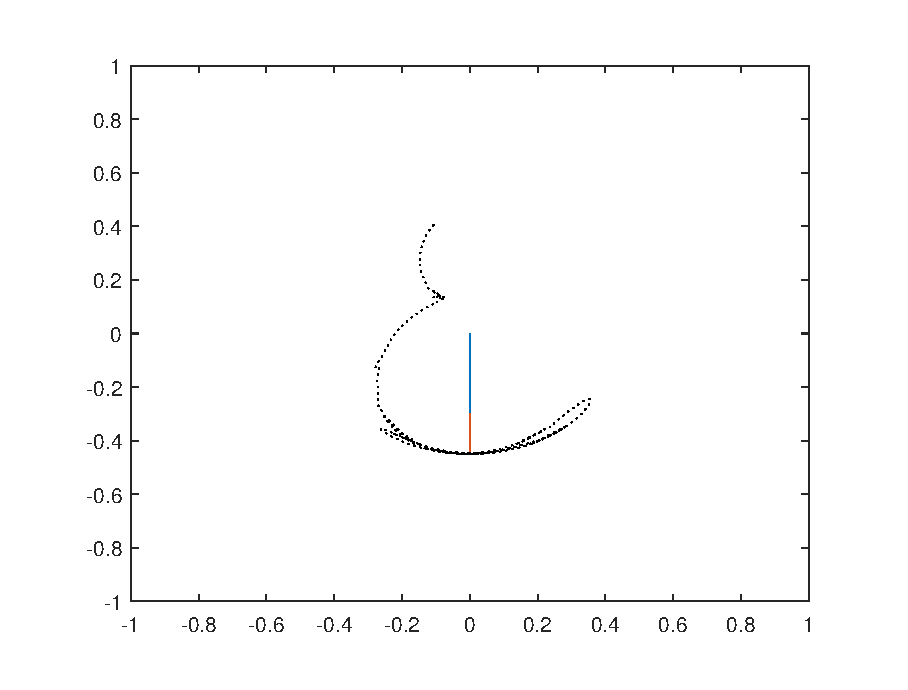
\includegraphics[width=0.4\textwidth]{6_f_0_menos10.eps}
	\caption{}
  \label{}
\end{figure}

Usando esta força cartesiana, sendo esta semelhante à força da gravidade, e uma vez que a força é exercida ao longo do eixo dos yy, o efeito sentido é o mesmo que o da Força gravítica: o robô parte da posição inicial, caindo o braço e depois permanece numa posição de equilíbrio ao fim de algum tempo.
\linebreak

Caso 2: \begin{equation} F_c = \begin{bmatrix}
10 & 0
\end{bmatrix}
^{T}
\end{equation}

\begin{figure}[H]
	\centering
	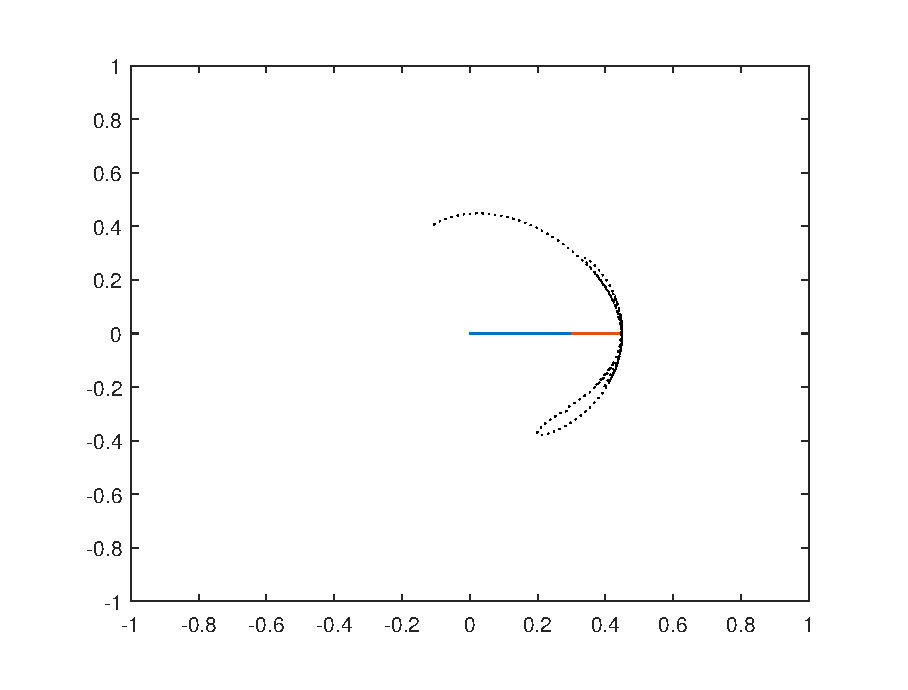
\includegraphics[width=0.4\textwidth]{6_f_10_0.eps}
	\caption{}
  \label{}
\end{figure}

Neste caso, a força é exercida segundo o eixo dos xx, observando-se uma força de equilíbrio segundo este mesmo eixo.
\\

Caso 3: \begin{equation} F_c = \begin{bmatrix}
10 & -10
\end{bmatrix}
^{T}
\end{equation}

\begin{figure}[H]
	\centering
	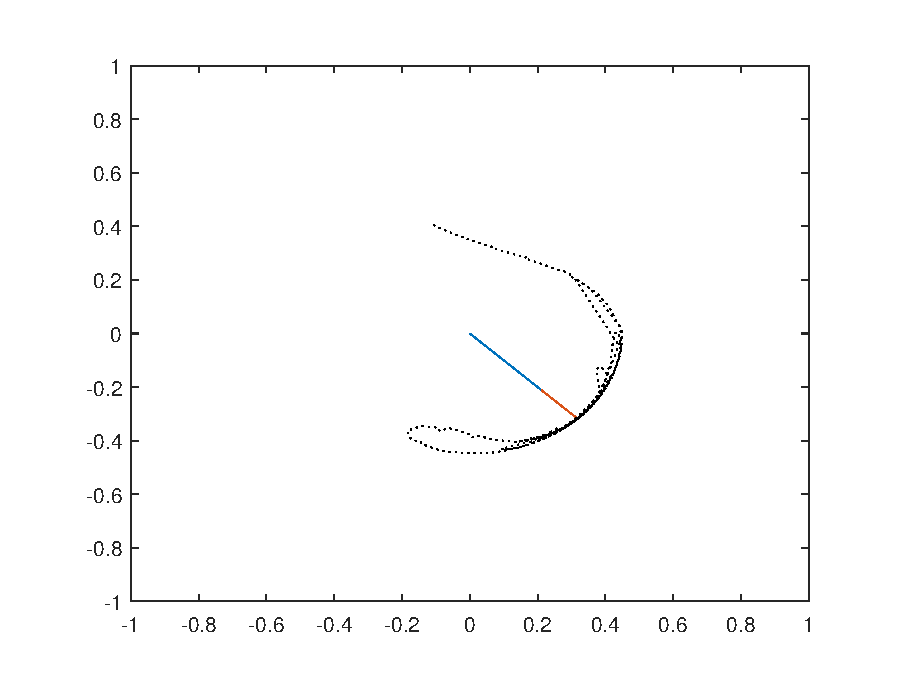
\includegraphics[width=0.4\textwidth]{6_f_10_menos10.eps}
	\caption{}
  \label{}
\end{figure}

Neste caso, a força aplicada é uma combinação das duas anteriores, tendo assim duas contribuições: uma segundo o eixo dos xx e uma segundo o eixo dos yy. 
\\

Conclui-se, então, que com a compensação de gravidade activa, o end-effector desloca-se na direcção da força aplicada. No entanto, como não está implementado nenhum controlador, existe oscilação no movimento e presença de \textit{overshoot}.

De forma a corrigir isto, a ideia é implementar um controlador que, tendo em conta uma posição desejada, aplique um binário de forma a que o robô se mova para essa mesma posição.

Se não se atenuasse a oscilação e o \textit{overshoot} numa situação real, o robô poderia não desempenhar as suas tarefas com uma precisão suficientemente boa para uma cirurgia. 

\subsection{Controlo P e PD no espaço de tarefa}

Os esquemas de controlo têm como objectivo remover o \textit{overshoot} e oscilação, sendo considerada uma posição desejada associada a uma trajectória elíptica com frequência $\frac {1}{4}$Hz e centrada em (0.25,0.2), e com $m_x$= 0.12 e $m_y$ = 0.07.
Sendo $X_d$ a posição desejada e $\omega=2\pi f$:

\begin{equation}
X_d=
\begin{bmatrix}
0.25 +  0.12cos(\omega t)\\
0.2 + 0.07sin(\omega t)
\end{bmatrix}
\end{equation}

No caso do controlo PD, o torque total corresponde ao torque de controlo, uma vez que todas as outras forças externas são nulas.

\begin{equation}
    \tau_c = J^{T}[K_d(\dot{X}_d -\dot{X}) + K_p(X_d -X)]
\end{equation}

Utilizando a lei de controlo referida na equação \ref{eqTauc}, obtemos:

\begin{equation}
    F_c=K_d(\dot{X}_d - \dot{X}) + K_p(X_d - X)
\end{equation}

Num controlo PD, $K_p$ e $K_D$ são os ganhos proporcional (P) e derivativo (D), respectivamente.
O esquema PD usado para fazer a simulação é:

\begin{figure}[H]
	\centering
	\includegraphics[width=0.3\textwidth]{esquemaPD.png}
	\caption{\cite{Cortesão}}
  \label{}
\end{figure}

Foram usados diferentes conjuntos de ganhos $K_p$ e $K_d$.

Caso 1: $K_p$=20 e $K_D$=20  
\begin{figure}[H]
	\centering
	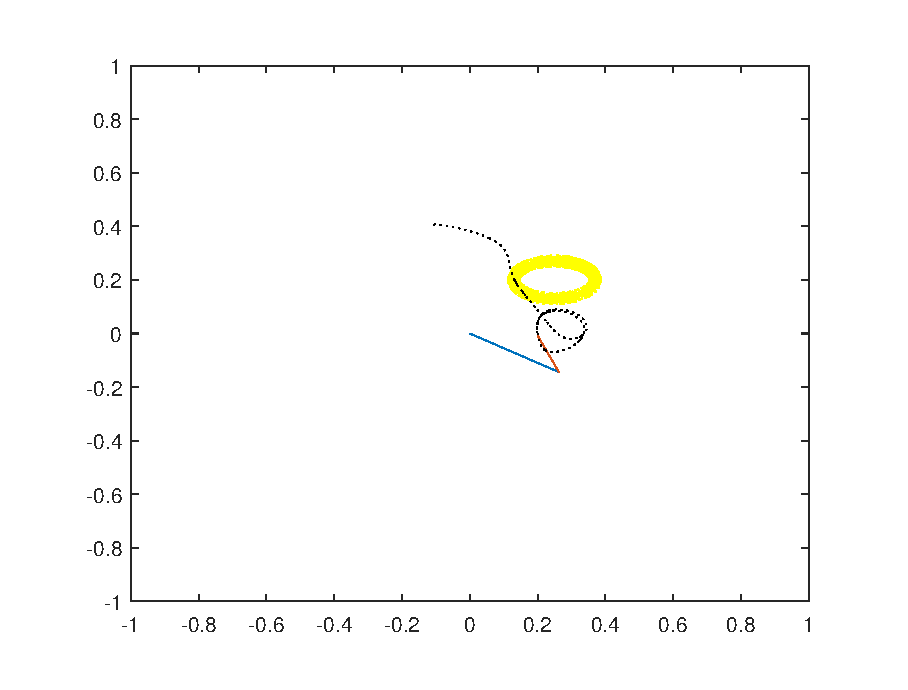
\includegraphics[width=0.4\textwidth]{7pd_ganhos_20_20.eps}
	\caption{}
  \label{}
\end{figure}

Para valores baixos de $K_p$ e $K_D$, a posição do \textit{end-effector} não consegue acompanhar a trajectória pretendida, havendo um desvio acentuado. Isto porque há um desfasamento acentuado entre $X_d$ (a trajectória) e X (a posição actual), fazendo com que o \textit{end-effector} corte a trajectória. Desta forma, o vetor ($X_d$-X) não segue a trajectória pretendida.
\linebreak


Caso 2:  $K_p$=120 e $K_D$=70

\begin{figure}[H]
	\centering
	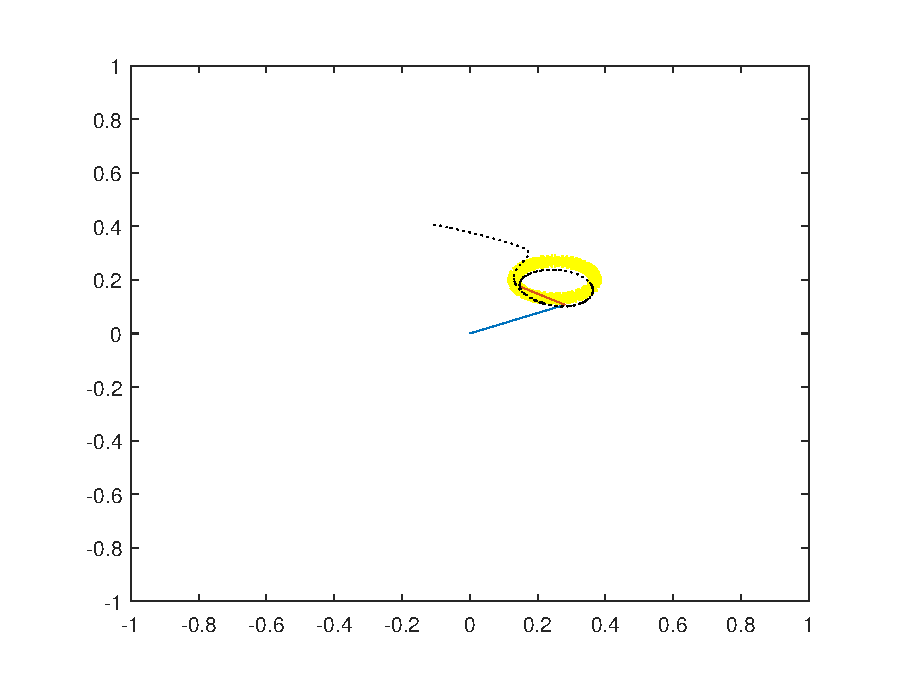
\includegraphics[width=0.4\textwidth]{7pd_ganhos_120_70.eps}
	\caption{}
  \label{}
\end{figure}

De forma a diminuir-se o desfasamento entre a trajectória e a posição atual, aumentou-se o $K_p$, aumentando a velocidade do robô. É necessário ter em atenção que um valor de $K_p$ excessivo pode levar à ocorrência de oscilações.
Neste caso, a posição do \textit{end-effector} já se aproxima mais da trajectória pretendida.
\\

Caso 3: $K_p$=20 e $K_D$=1000

\begin{figure}[H]
	\centering
	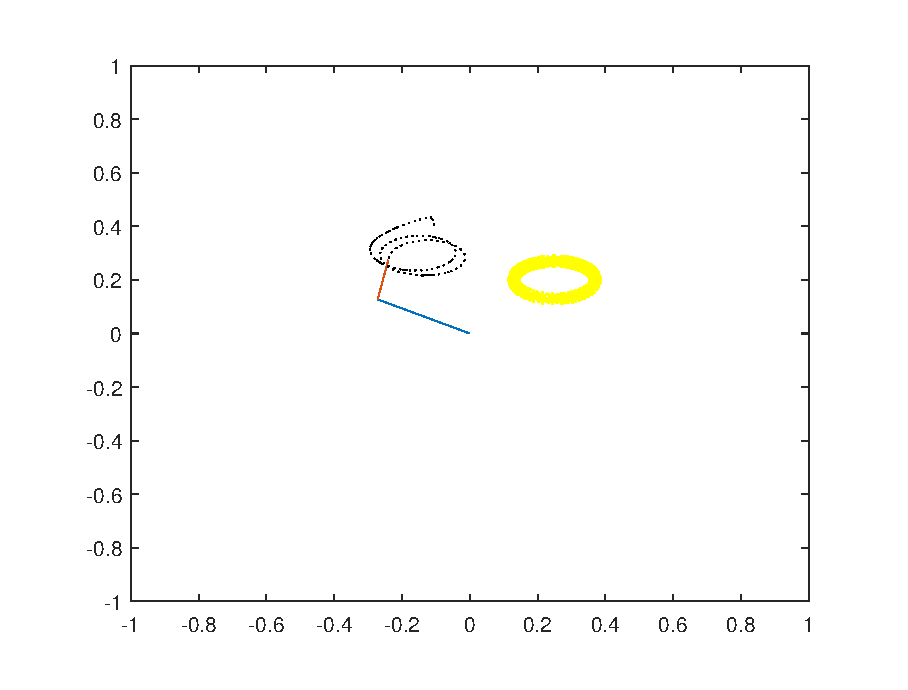
\includegraphics[width=0.4\textwidth]{7pd_ganhos_20_1000.eps}
	\caption{}
  \label{}
\end{figure}

Neste caso, experimentou-se usar um valor baixo de $K_p$ e um valor alto de $K_D$. O que sucedeu foi que, embora a velocidade fosse aumentada, houve um desfasamento grande entre a posição do \textit{end-effector} e da trajectória.
\\

Caso 4: $K_p$=1000 e $K_D$=20

\begin{figure}[H]
	\centering
	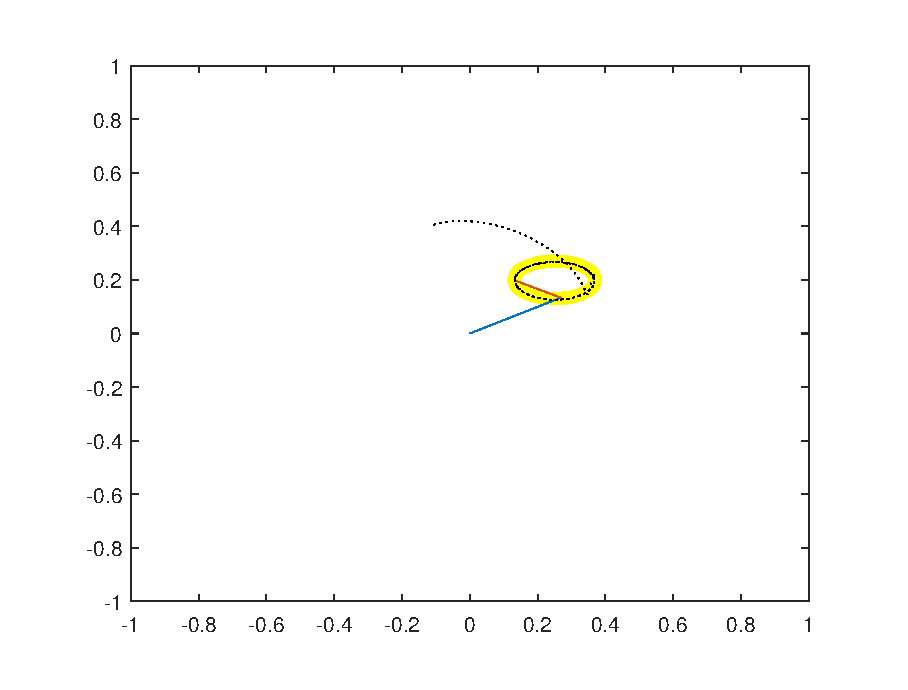
\includegraphics[width=0.4\textwidth]{7pd_ganhos_1000_20.eps}
	\caption{}
  \label{}
\end{figure}

Alterando novamente os valores, incrementando o valor de $K_p$ e diminuindo $K_D$, obtivemos a trajectória que melhor se aproxima da trajectória definida. 
\\
 
A partir da observação das trajectórias do robô para os diferentes casos, concluímos que quanto maior a razão entre os ganhos $K_p$ e $K_D$, mais se aproxima a posição actual da trajectória pretendida, sendo que o valor de $K_p$ terá que ser superior ao valor de $K_D$. 
Ganhos de $K_p$ e $K_D$ baixos, desfavorecem a aproximação entre a posição do \textit{end-effector} e a posição pretendida.
\linebreak

Testando agora uma trajectória vertical:
\\

Caso 1:  $K_p$=100 e $K_D$=60

\begin{figure}[H]
	\centering
	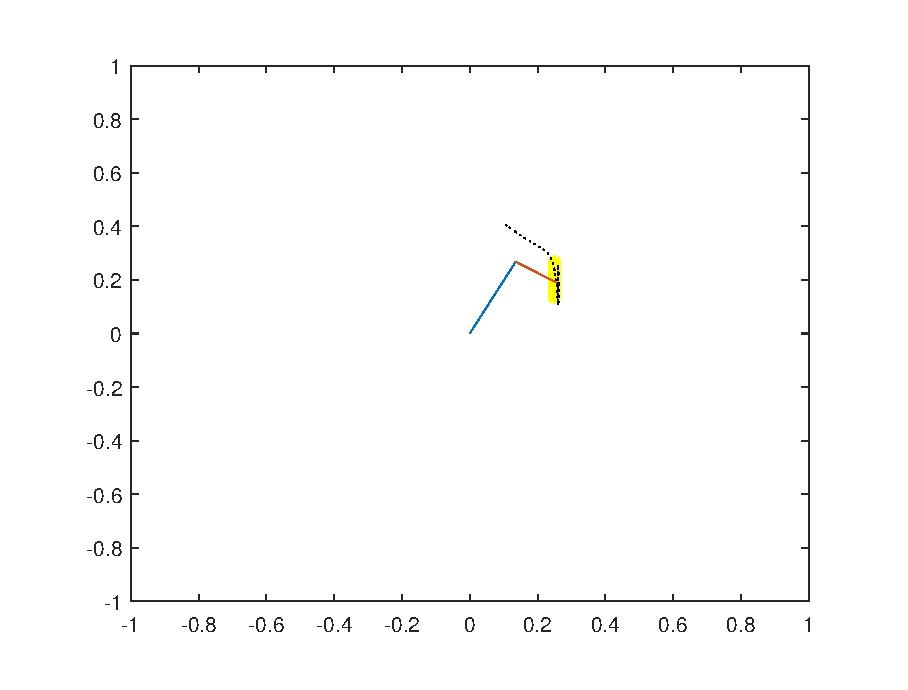
\includegraphics[width=0.4\textwidth]{7_vertical_pd_ganhos_100_60.eps}
	\caption{}
  \label{}
\end{figure}

Caso 2:  $K_p$=100 e $K_D$=10

\begin{figure}[H]
	\centering
	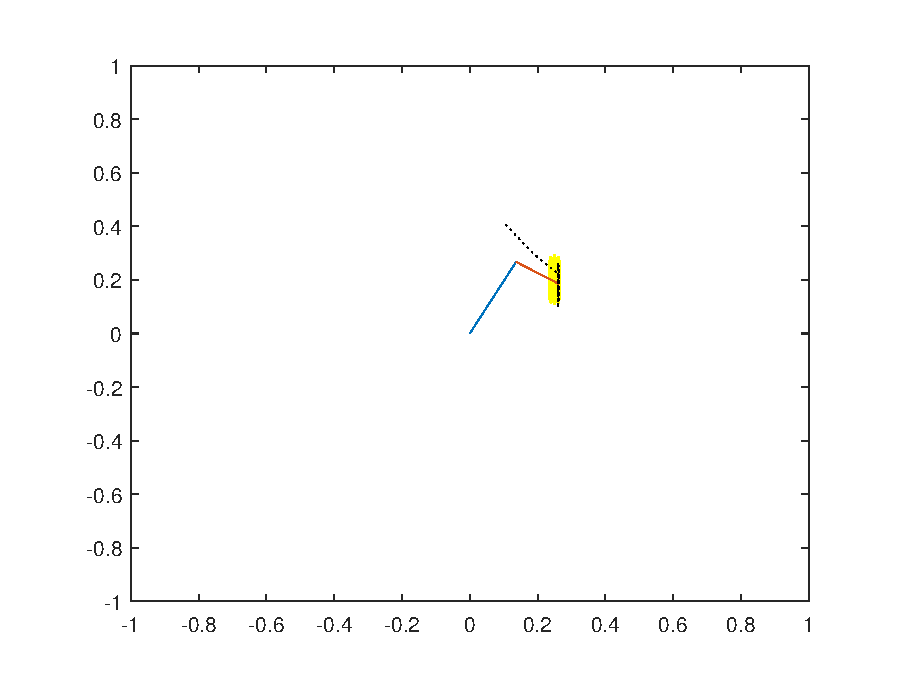
\includegraphics[width=0.4\textwidth]{7_vertical_pd_ganhos_100_10.eps}
	\caption{}
  \label{}
\end{figure}

Usando uma trajectória vertical, também se constata que quanto maior for a razão entre os ganhos $K_p$ e $K_D$, maior a aproximação da posição à trajectória desejada.
\\

Testando agora o esquema de controlo P, igualamos $K_D$ a 0.
\\

Caso 1: $K_p$=1000

\begin{figure}[H]
	\centering
	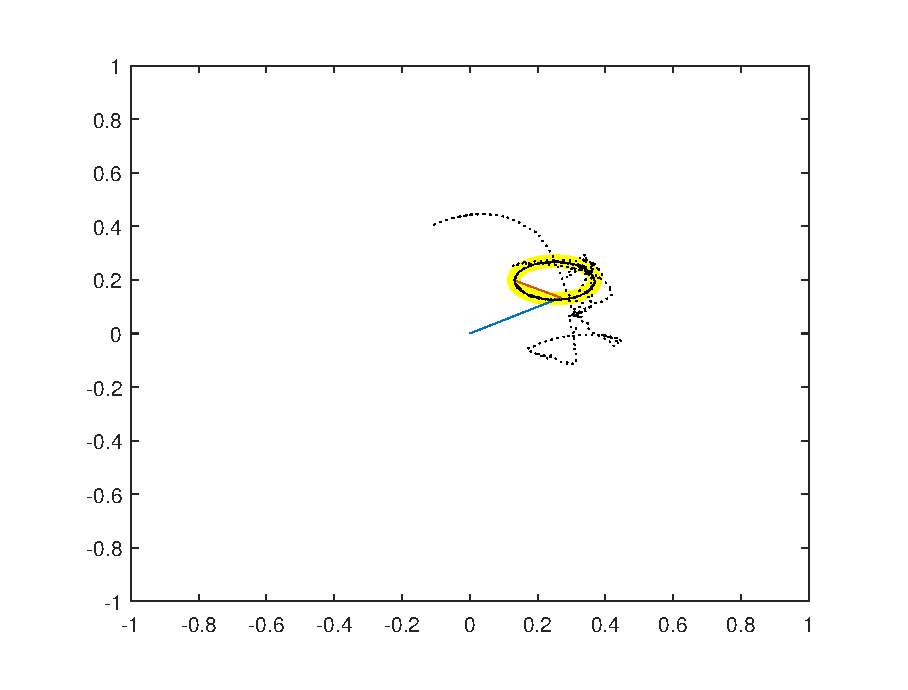
\includegraphics[width=0.4\textwidth]{7_p_ganho1000.eps}
	\caption{}
  \label{}
\end{figure}

Caso 2: $K_p$=100

\begin{figure}[H]
	\centering
	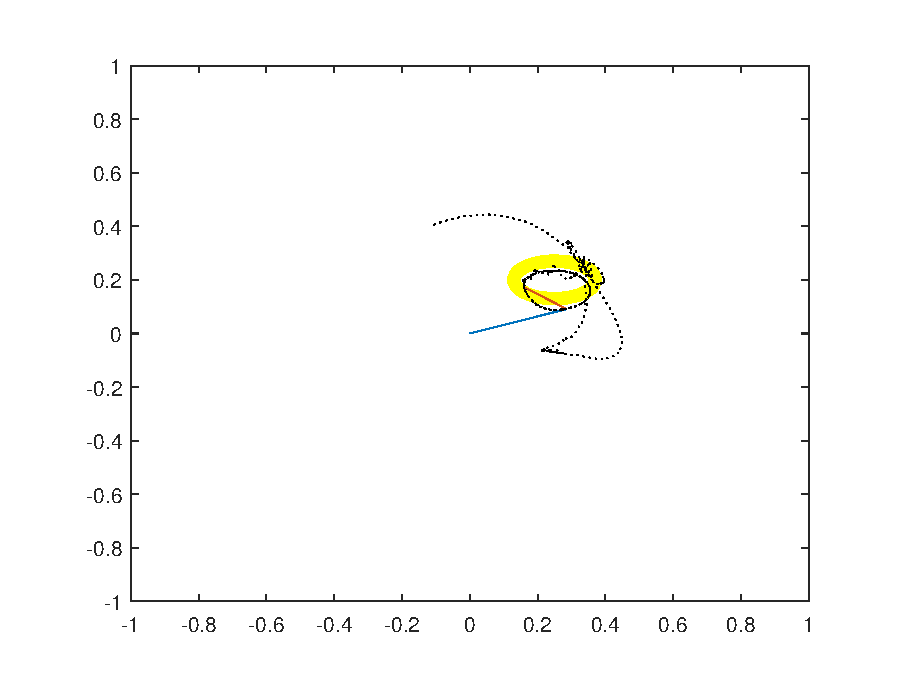
\includegraphics[width=0.4\textwidth]{7_p_ganho100.eps}
	\caption{}
  \label{}
\end{figure}

Caso 3: trajectória vertical com $K_p$=100

\begin{figure}[H]
	\centering
	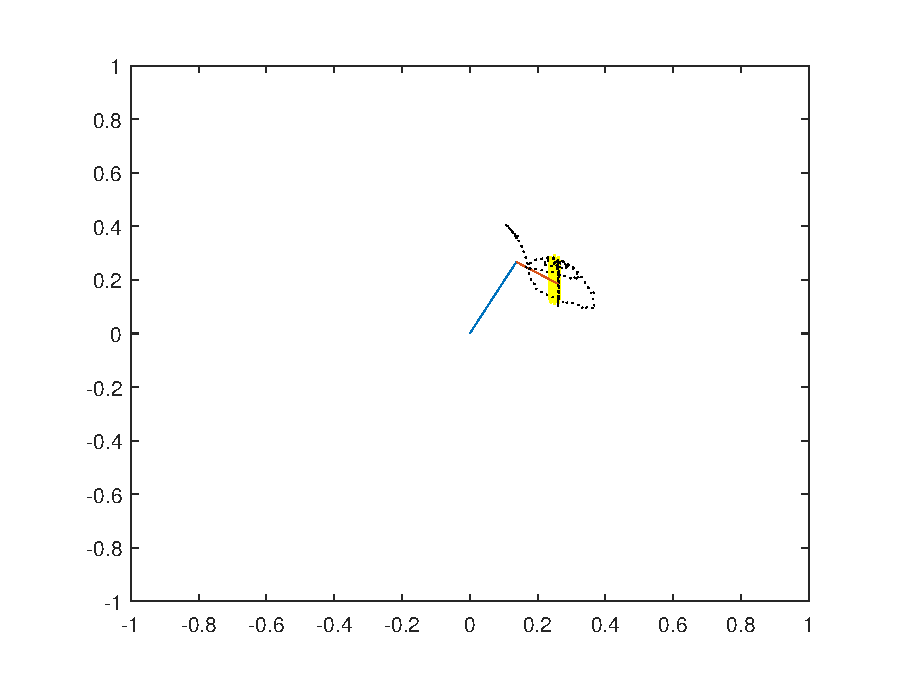
\includegraphics[width=0.4\textwidth]{7_vertical_p_ganho100.eps}
	\caption{}
  \label{}
\end{figure}


Através da presença de controlo P, é possível verificar-se que o \textit{end-effector} se aproxima mais rapidamente da trajectória desejada quanto maior for $K_p$.~No entanto, ocorrem oscilações tanto maiores quanto maior for a referência de posição $K_p$. O ganho $K_p$ introduz uma força que minimiza a diferença entre a posição do \textit{end-effector} e a posição desejada. 
Em contexto clínico, é importante a existência do controlo PD, pois a instabilidade inicial do controlo P pode causar danos nos tecidos envolventes.
\\

Foi ainda testado um modelo dinâmico. As não-linearidades são anuladas devido à utilização de técnicas de linearização por feedback dissociadas do controlo. Assim, é garantida a consistência da resposta dinâmica. 
Um modelo dinâmico pode ser visto como o "coração" de um algoritmo de controlo sofisticado.

Para garantir a linearização, a lei de controlo é, neste caso:

\begin{equation}
    M(q)J^{-1}(w-\dot{J}\dot{q}) + v(\dot{q},q) + g(q) = \tau_c
\end{equation}

sendo,

\begin{equation}
   w = K_p(X_d - X) + K_d(\dot{X}_d - \dot{X})
\end{equation}

O esquema PD usado para fazer a simulação do modelo dinâmico foi:

\begin{figure}[H]
	\centering
	\includegraphics[width=0.4\textwidth]{esquema_7_din.png}
	\caption{\cite{Cortesão}}
  \label{}
\end{figure}


Para o caso em que $K_p$=1000 e $K_D$=20, obtivemos:

\begin{figure}[H]
	\centering
	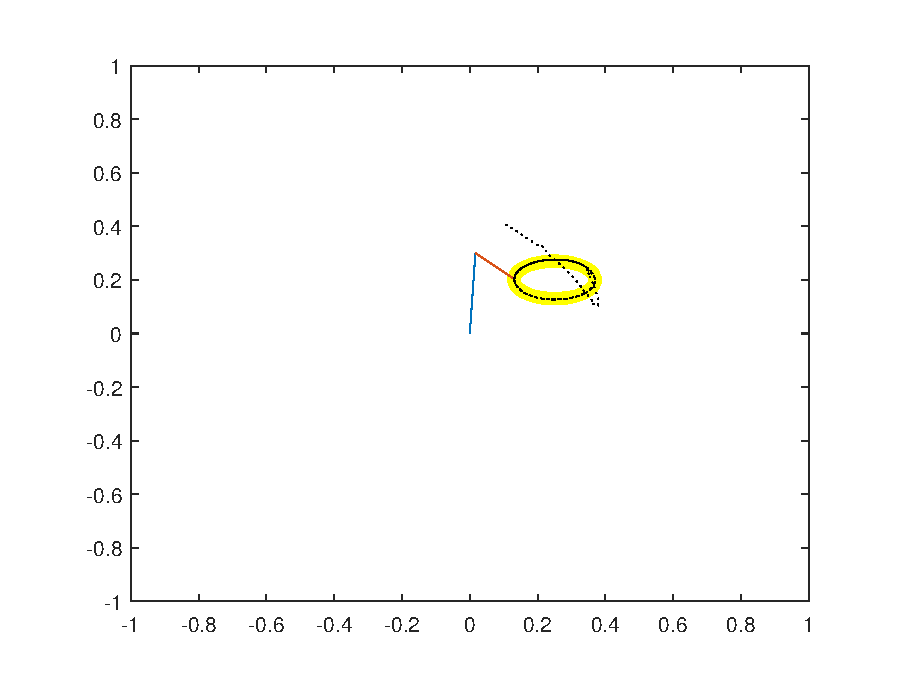
\includegraphics[width=0.4\textwidth]{7_versao1.eps}
	\caption{}
  \label{}
\end{figure}

O uso do modelo dinâmico leva a uma maior robustez no controlo da posição. 


\subsection{Controlo de complacência para interacções com o osso}

Neste ponto, pretende-se analisar a interacção do robô com o osso, de forma a estudar o comportamento do robô. Considerou-se um osso horizontal virtual com uma certa rigidez. Na nossa simulação, desenhamos o osso como sendo um semi-círculo, simulando assim, a interacção com a epífise de um osso longo.

\begin{figure}[H]
	\centering
	\includegraphics[width=0.4\textwidth]{parts-long-bone.png}
	\caption{Anatomia de um osso longo \cite{Sleewee}.}
  \label{}
\end{figure}
\linebreak
O esquema de controlo de complacência usado foi o seguinte:

\begin{figure}[H]
	\centering
	\includegraphics[width=0.4\textwidth]{Diapositivo1.PNG}
	\caption{\cite{Cortesão}}
  \label{}
\end{figure}

O controlo de interacção é importante para garantir que o robô não provoca danos no tecido, sendo essencial para situações em que seja necessário controlo de força e precisão.
O controlo de complacência baseia-se no cálculo da força em oposição, não existindo necessidade de qualquer tipo de sensor de força. 

Define-se, então, uma barreira de contacto, considerando que o \textit{end-effector} se comporta como se estivesse ligado a uma mola com uma certa rigidez.

Em ambiente cirúrgico, pretende-se operar
apenas uma zona de interesse sem danificar os tecidos adjacentes. Assim, uma solução para uma manipulação segura pode ser impôr alguma complacência e rigidez ao controlo do robô.
A rigidez é ao nível das juntas do robô, condicionando a força que o robô exerce sobre o meio. 
Seja $F_e$ a força que o robô aplica sobre o ambiente e $K_c$ a rigidez imposta durante o movimento, tem-se:

\begin{equation}
    F_e = K_cJdq = K_cdX_c
\end{equation}

É este o princípio do Active Stiffness Control. As forças do robô relacionam-se com os deslocamentos diferenciais
em redor do ponto de equilíbrio através da rigidez $K_c$.
\\

Considerou-se o osso a partir da posição x=0.25. 
\linebreak

O torque que o ambiente aplica no robô define-se por:

\begin{equation}
    \tau_e=-J^{T}F_e
\end{equation}
\linebreak

No espaço de tarefa, a lei de controlo em espaço livre, com complacência é:

\begin{equation}
    \tau_c=J^{T}[K_p(X_d - X) - K_D\dot{X}] + g(q) + J^{T}F_{phys}
\end{equation}
\linebreak

$F_{phys}$ sendo a força exercida pelo médico no \textit{end-effector}.
\\

Em contacto, ou seja, na presença da força $F_e$ aplicada pelo ambiente:

\begin{equation}
\resizebox{.4\textwidth}{!}{
   $ \tau = J^{T}[K_p(X_d - X) - K_D\dot{X}] - J^{T}F_e + g(q) + J^{T}F_{phys}$}
\end{equation}
\linebreak

Para o caso em que está em contacto, ou seja, quando chega ao osso e este exerce uma força sobre o robô, $F_e$ =
$K_e$(X-$X_e$). Em espaço livre esta força é nula.

O robô também possui uma determinada rigidez ($K_p$) em que 
\begin{equation}
    F_e = \frac{K_p K_e}{K_p + K_e}(X_d - X_e)
\end{equation}

Assim, esta é a força correspondente ao resultado de duas molas em série, tendo cada uma das molas uma rigidez diferente.

O valor escolhido de $K_p$ terá que garantir a presença de rigidez e velocidade de resposta, e também terá que ser baixo o suficiente para não colocar em risco o paciente ou o médico. 
O valor de $K_D$ deve impedir que ocorra \textit{overshoot}.

$K_p$ terá apenas influência segundo a componente dos yy, $K_e$ terá exclusivamente a nível da componente dos xx, e $K_D$ em ambas as componentes.

A condição humana dificilmente permite a aplicação de forças perfeitamente lineares pelo que, por vezes são aplicadas forças com ligeiras oscilações.
No entanto, nestas simulações foi considerado para a Força exercida pelo médico no robô:

\begin{equation}
F_{phys} =
    \begin{bmatrix}
    10 \\
    0
    \end{bmatrix}
\end{equation}

\linebreak

De forma a que o robô penetre apenas um bocado no osso, usamos os valores:

\begin{equation}
K_e =
    \begin{bmatrix}
    200 & 0 \\
    0 & 0
    \end{bmatrix}
\end{equation}

\begin{equation}
K_p =
    \begin{bmatrix}
    0 & 0 \\
    0 & 2000
    \end{bmatrix}
\end{equation}

\begin{equation}
K_D =
    \begin{bmatrix}
    10 & 0 \\
    0 & 10
    \end{bmatrix}
\end{equation}

\begin{figure}[H]
	\centering
	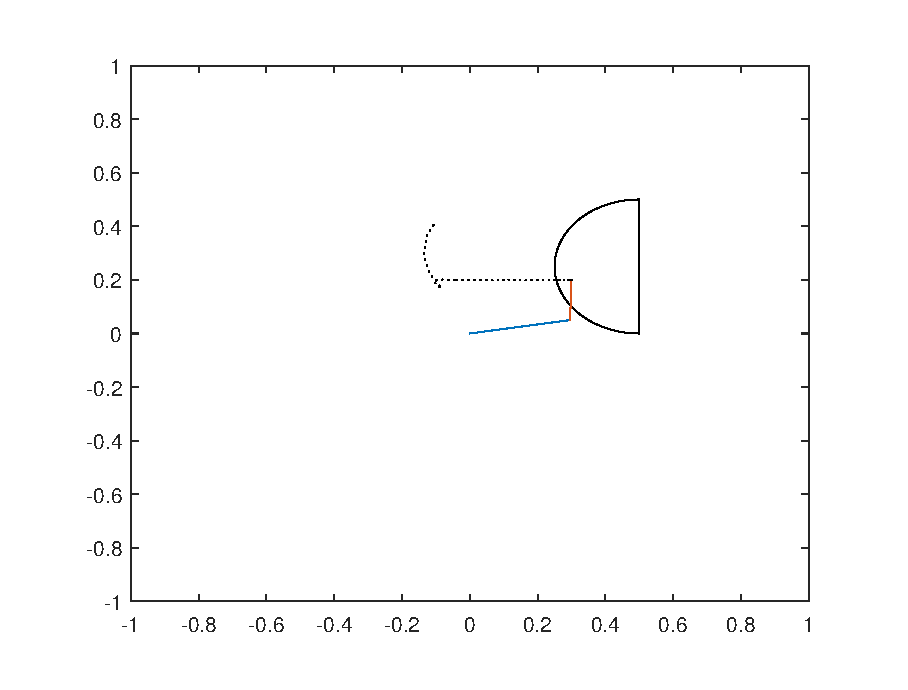
\includegraphics[width=0.4\textwidth]{neste_penetra_lol.eps}
	\caption{}
  \label{}
\end{figure}

Foi possível penetrar no osso, uma vez que a rigidez do osso era inferior à rigidez do robô.

Agora, tentando que o robô não penetre no osso, usamos os valores:

\begin{equation}
K_e =
    \begin{bmatrix}
    2000 & 0 \\
    0 & 0
    \end{bmatrix}
\end{equation}

\begin{equation}
K_p =
    \begin{bmatrix}
    0 & 0 \\
    0 & 200
    \end{bmatrix}
\end{equation}

\begin{equation}
K_D =
    \begin{bmatrix}
    10 & 0 \\
    0 & 10
    \end{bmatrix}
\end{equation}

\begin{figure}[H]
	\centering
	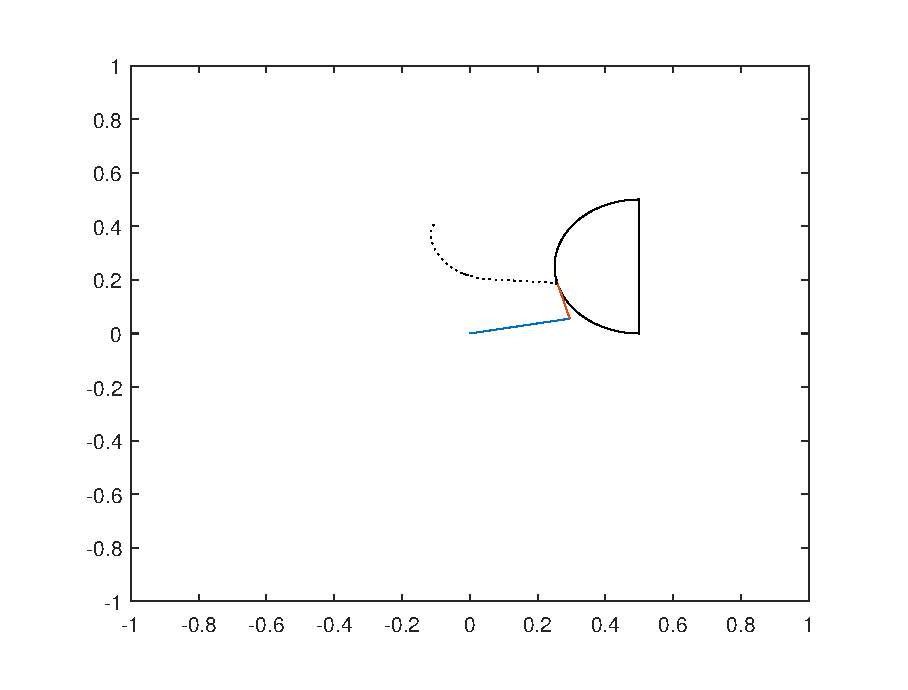
\includegraphics[width=0.4\textwidth]{8_naopenetra.eps}
	\caption{}
  \label{}
\end{figure}
Assim, aumentando a rigidez do osso, o robô já não consegue penetrar no osso. 
Daqui conclui-se que, se $K_p$ >> $K_e$, o robô é muito rígido e atravessa o osso, chegando próximo da posição desejada com mais facilidade.
Por outro lado, se $K_p$ << $K_e$, o robô tem mais dificuldade em avançar pela parede, ficando mais afastado da posição pretendida.



Agora, testando uma força aplicada pelo médico maior:

\begin{equation}
F_{phys} =
    \begin{bmatrix}
    50 \\
    0
    \end{bmatrix}
\end{equation}

\begin{figure}[H]
	\centering
	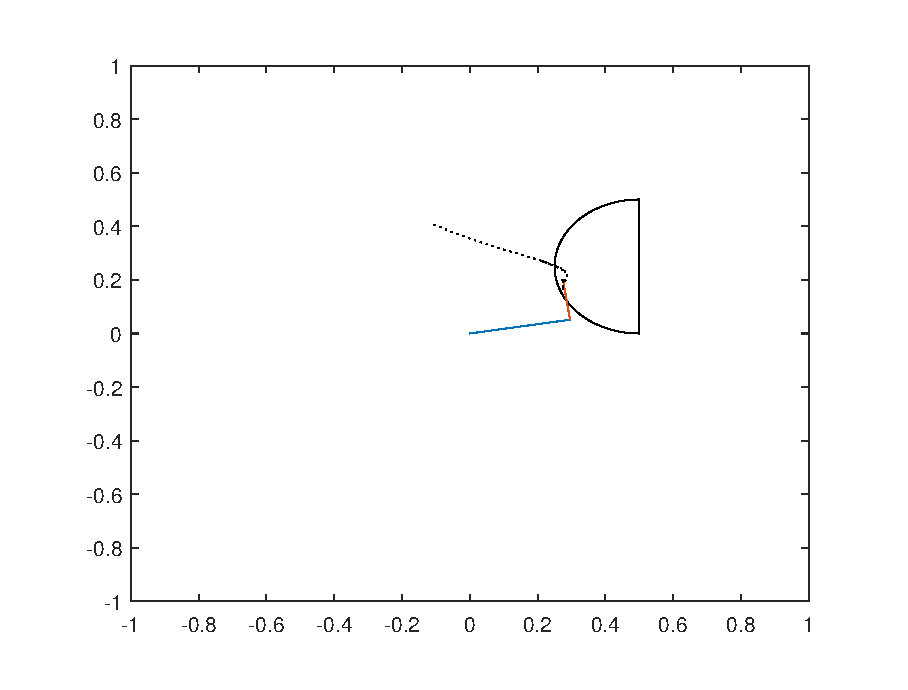
\includegraphics[width=0.4\textwidth]{8_fphys_50_0.eps}
	\caption{}
  \label{}
\end{figure}

Aumentando $F_{phys}$, e considerando os mesmos valores de $K_D$, $K_p$ e $K_e$, reparamos que o robô consegue avançar em maior profundidade no osso. Conclui-se, assim, que a aplicação de uma força cartesiana maior (uma vez que a força exercida pelo médico é maior), favorece o movimento sobre a trajectória pretendida nas mesmas condições de rigidez.


\subsection{Controlo de Impedância}

O controlo de impedância é uma generalização do controlo de complacência, em que a dinâmica do robô em situações de contacto é especificada em função de características dinâmicas desejadas de um sistema massa-mola-amortecedor.

Pretende-se que o robô execute um movimento horizontal do \textit{end-effector} até encontrar a superfície do osso e atingir uma dada posição de equilíbrio.
O constrangimento horizontal foi executado com a aplicação de uma parede virtual para restringir a trajectória. Ao chegar à superfície do osso, o robô é sujeito a uma nova impedância e à restrição imposta por uma nova parede virtual vertical.

A velocidade do \textit{end-effector} $\dot{X}$ e a força aplicada pelo robô na interacção (\textit{Fe}) estão relacionadas por uma impedância Z, com:

\begin{equation}
-F_e(s) = Z(s)\dot{X}(s)
\end{equation}

\begin{equation}
sZ(s) = As^{2} + Ds + K
\end{equation}

onde A, K e D são os parâmetros desejados do sistema massa-mola-amortecedor. A dinâmica do robô em contacto é dada por:

\begin{equation}
M(q) + C(q,\dot{q})\dot{q} + g(q) + J^{T}F_e = \tau
\end{equation}

A lei de controlo pode ser definida como:

\begin{equation}
\tau_c = MJ^{-1}(w-\dot{J}\dot{q}) + v(q,\dot{q}) + g(q) + J^{T}F_e
\end{equation}

de forma a se obter o comportamento do robô desejado, tem-se:

\begin{equation}
\tau_c = MJ^{-1}(w-\dot{J}\dot{q}) + v(q,\dot{q}) + g(q) + J^{T}F_e
\end{equation}

Considerando que não existe \textit{inertia~shaping} (uma vez que o termo mássico é difícil de implementar), assume-se que:

\begin{equation}
A^{-1} = JM^{-1}J^{T}
\end{equation}

Assim, os termos de $F_e$ anulam-se, não sendo necessário utilizar sensores de força.
\\

O esquema usado para a simulação foi o seguinte:

\begin{figure}[H]
	\centering
	\includegraphics[width=0.4\textwidth]{esquema_9.png}
	\caption{Esquema de controlo de impedância \cite{Cortesão}.}
  \label{}
\end{figure}

Foi considerada uma força aplicada pelo médico ($F_{phys}$), à semelhança do ponto anterior. 
Considerou-se, então, para a componente x, 10N e para a componente y, uma representação dos tremores (oscilações), com uma amplitude de 1 e frequência de 2$\pi$.

Considerou-se, ainda, para a matriz correspondente ao amortecimento:

\begin{equation}
D =
    \begin{bmatrix}
    15 & 0\\
    0 & 15
    \end{bmatrix}
\end{equation}

Considerando então tremores: 

\begin{figure}[H]
	\centering
	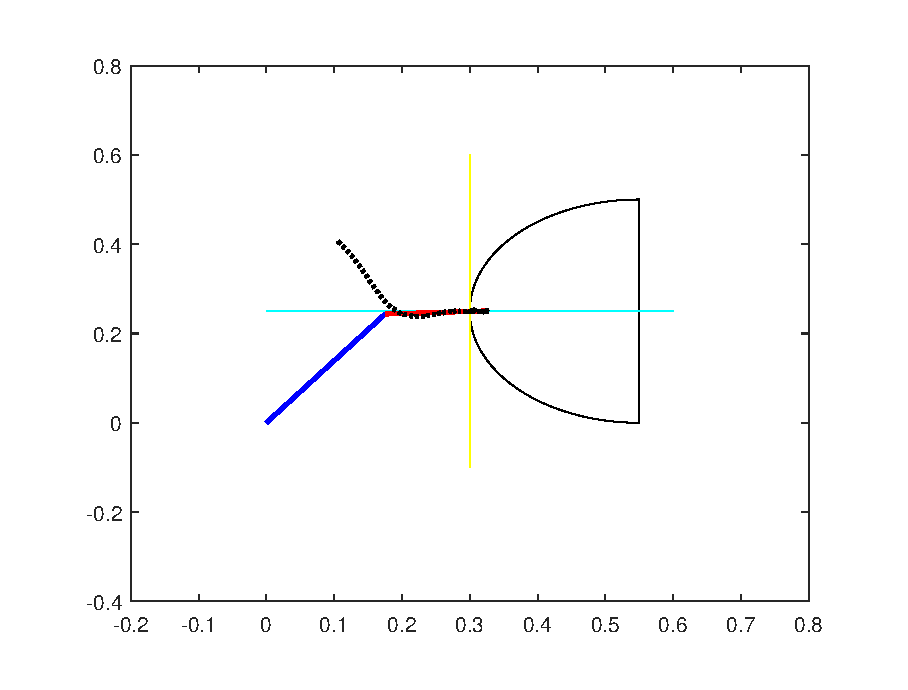
\includegraphics[width=0.4\textwidth]{9_oscil_ke200kp2000.eps}
	\caption{$K = \left[0~0 ;0~2000 \right]$ e $K_e = \left[200~0 ;0~0 \right] $.}
  \label{menorp}
\end{figure}

Para o mesmo caso anterior, aumentando o termo em y da matriz de D, a oscilação pode ser diminuída. Assim, os tremores do médico podem ser controlados, de maneira a que não haja riscos acrescidos para o paciente.

Assim, a partir daqui consideramos a força exercida pelo médico como: 

\begin{equation}
F_{phys} =
    \begin{bmatrix}
    10\\
    0
    \end{bmatrix}
\end{equation}

Testamos alterar os termos de K e $K_e$, para tirarmos conclusões acerca da sua variação:

\begin{figure}[H]
	\centering
	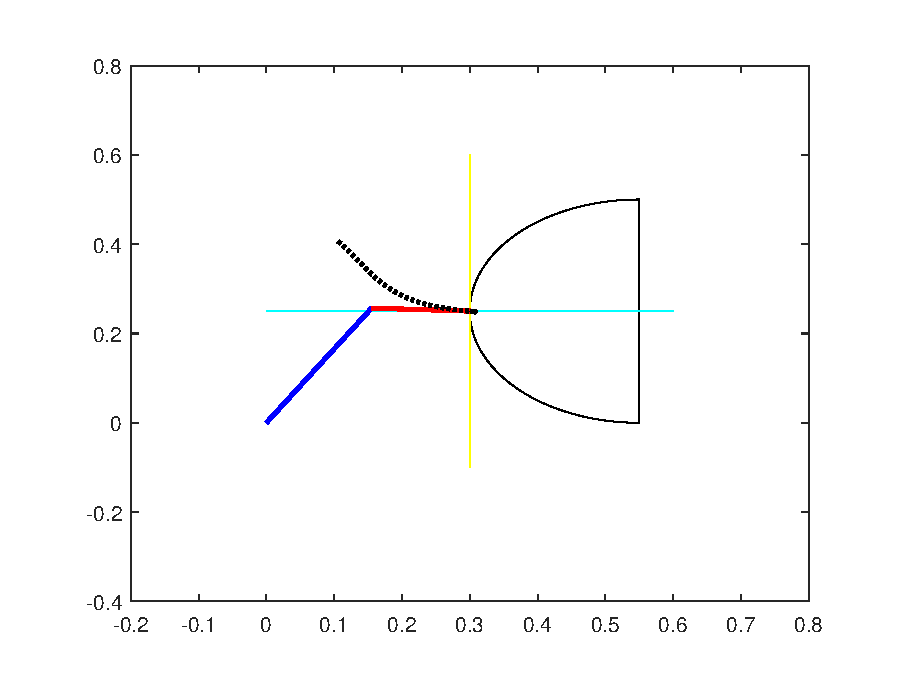
\includegraphics[width=0.4\textwidth]{9_ke2000_kp200_fm.eps}
	\caption{$K = \left[0~0 ;0~200 \right]$ e $K_e = \left[2000~0 ;0~0 \right] $.}
  \label{menorp}
\end{figure}

\begin{figure}[H]
	\centering
	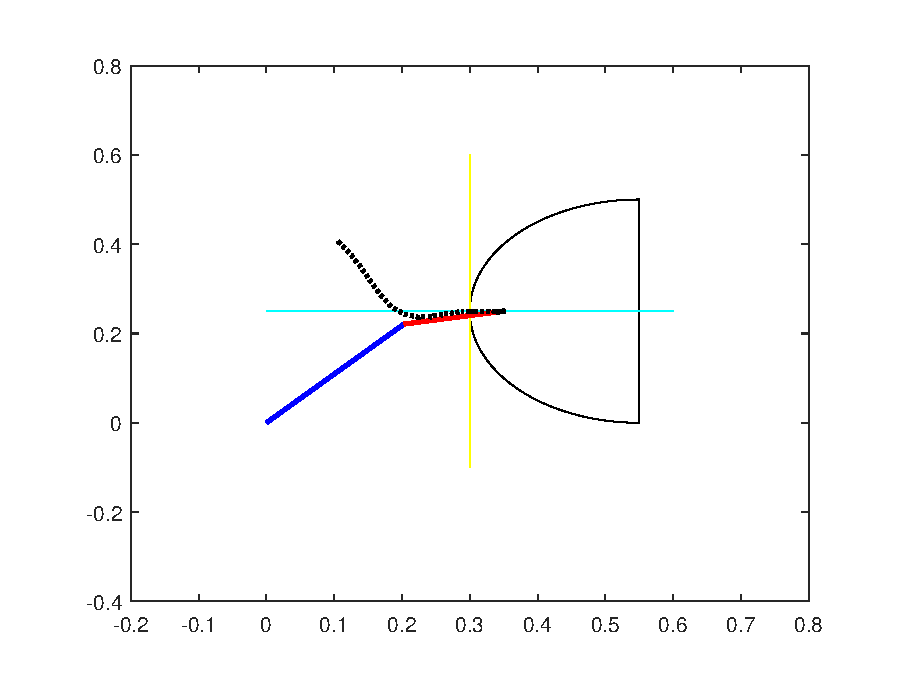
\includegraphics[width=0.4\textwidth]{9_ke200_kp2000_fm.eps}
	\caption{$K = \left[0~0 ;0~2000 \right]$ e $K_e = \left[200~0 ;0~0 \right] $.}
  \label{maiorp}
\end{figure}


Nas condições de um aumento do K, temos uma aceleração maior, assim como um aumento da força de contacto do robô. Sendo assim, os valores da matriz D (valores de amortecimento) são necessários para compensar tais acréscimos e garantir a segurança do paciente.

Das imagens \ref{menorp} e \ref{maiorp} podemos inferir que quanto maior o $K_e$ e menor o K, menor é a capacidade do robô em penetrar o osso, devido ao facto da rigidez do osso se sobressair à força do robô. A barreira que consideramos está à superfície do osso. 

O intuito de um robô cirurgião é, para além de facilitar o trabalho do médico durante o procedimento, amenizar os erros e riscos que o paciente está exposto, desta forma, deve-se garantir que os ganhos de controlo e as forças resultantes sejam ajustadas adequadamente, para que o robô possa mover-se de forma segura, porém manipulável.
 

\section{Trajectory Design}
 
 Neste ponto, considerou-se um robô de 3 links. Este robô apresenta um modelo  redundante, isto é, com um  grau de liberdade maior do que o espaço em que está inserido.

 Um robô redundante pode apresentar posturas diferentes para uma mesma posição do \textit{end-effector}, as quais são definidas pelos diferentes valores de $q$.
 
 A redundância do robô faz-se necessária para a manipulação do espaço nulo, afim de controlar os movimentos do robô e evitar, portanto, os órgãos vitais.
 
 Sendo assim, definiu-se uma postura desejada, próxima as juntas, a qual deu-se o nome de $q_d$. De seguida, aplicou-se um binário, o qual irá actuar apenas no espaço nulo, de forma a que a postura do robô aproxime-se da desejada, sem depender da posição do \textit{end-effector}.

Por se tratar de um robô redundante, a generalização inversa do Jacobiano é dada pela equação:

\begin{equation}
    J^{\#}=W^{-1}J^T(JW^{-1}J^T)^{-1}
    \label{eq3.78}
\end{equation}

Ao considerar que W=I , $J^{\#}$ pode ser chamada de pseudo inversa de \textit{Moore-Penrose}, uma vez que estamos a eliminar a dependência de $J^{\#}$ de parâmetros dinâmicos, e portanto:
\begin{equation}
    J^{\#}=J^T(JJ^T)^{-1}
\end{equation}
Sabendo que o erro da posição pode ser convertido em uma velocidade desejada tanto para o espaço de tarefas quanto para o espaço nulo, temos que:
\begin{equation}
    \dot{X}_d=K_p(X_d-X)
\end{equation}
Sendo $X_d$ a posição controlada pelo cirurgião, $K_p$ um ganho positivo e X a posição actual do robô.
E temos também:
\begin{equation}
    \dot{q}_0=K_q(q_{dp}-q)
\end{equation}
Na qual $K_q$ é uma constante positiva, $q_{dp}$ a postura desejada.
Sendo assim, para obter a posição desejada deve-se integrar a equação:
\begin{equation}
    \dot{q}_d= J^{\#}\dot{X}_d+(I-J^{\#}J)\dot{q}_0
\end{equation}
A qual é proveniente da equação \ref{eq3.78} com a equação:
\begin{equation}
     \dot{q}= J^{\#}\dot{X}+(I_{n\times n}-J^{\#}J)\dot{q}_0
\end{equation}
Para realizar a implementação e posteriormente a simulação, considerou-se que $l_1 = 1[m]$, $l_2=1[m]$ e $l_3=0.3[m]$. Também considerou-se os valores $K_p=K_d=10$.
\begin{figure}[H]
	\centering
	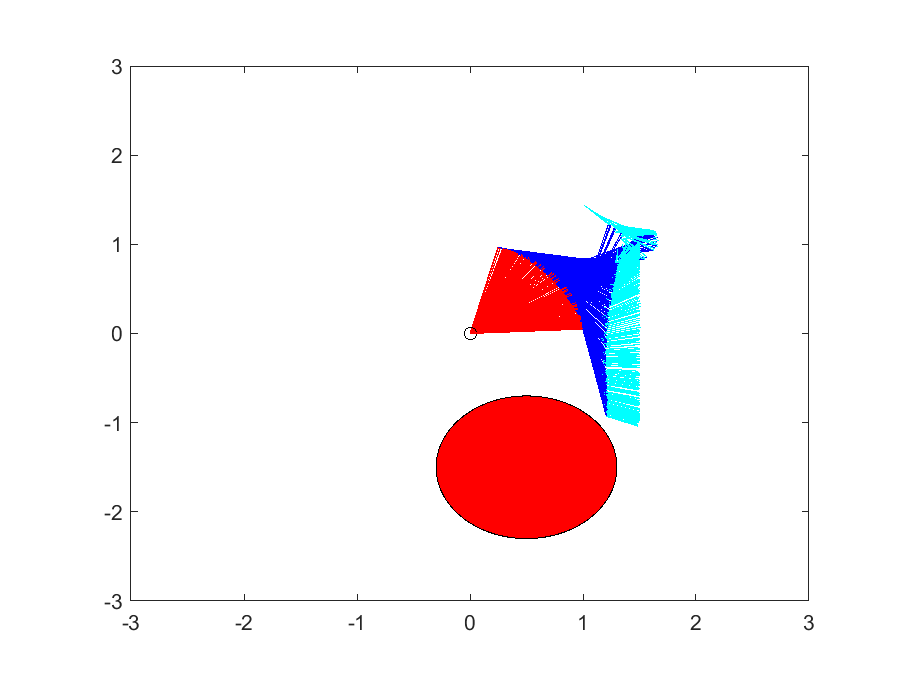
\includegraphics[width=0.35\textwidth]{qdp2.eps}
	\caption{Trajectória com controlo aplicado, em que $K_q=10$ e $q_{dp}=\left[\frac{80\pi}{180} ~\frac{-160\pi}{180}  ~
\frac{80\pi}{180}\right]^T $.}
\label{qdp2}
\end{figure}
Na figura \ref{qdp2} é verificável que ao se implementar as condições de controlo, o robô realiza a mesma trajectória sem colidir com àreas vitais(região representada a vermelho). Isto também é visível na figura \ref{qdp3}.
\begin{figure}[H]
	\centering
	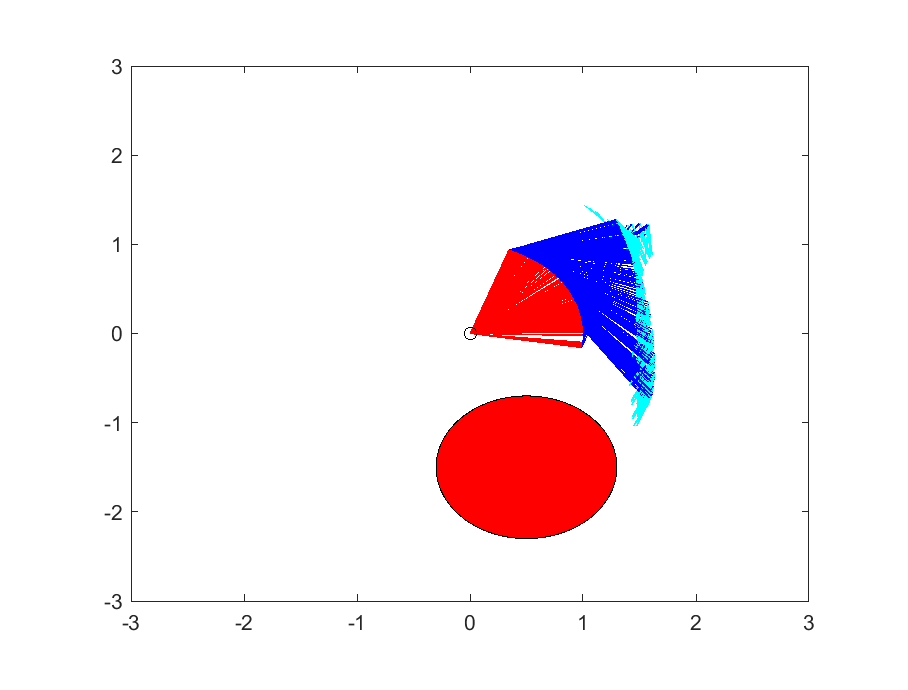
\includegraphics[width=0.35\textwidth]{qdp3.eps}
	\caption{Trajectória com controlo aplicado, em que $K_q=10$ e $q_{dp}=\left[\frac{\pi}{2} ~\frac{-\pi}{2}  ~\frac{-\pi}{2}\right]^T $.}
\label{qdp3}
\end{figure}
Se anularmos as condições de controlo, o robô atingirá as áreas vitais, como é observável na figura \ref{qdp1}.
\begin{figure}[H]
	\centering
	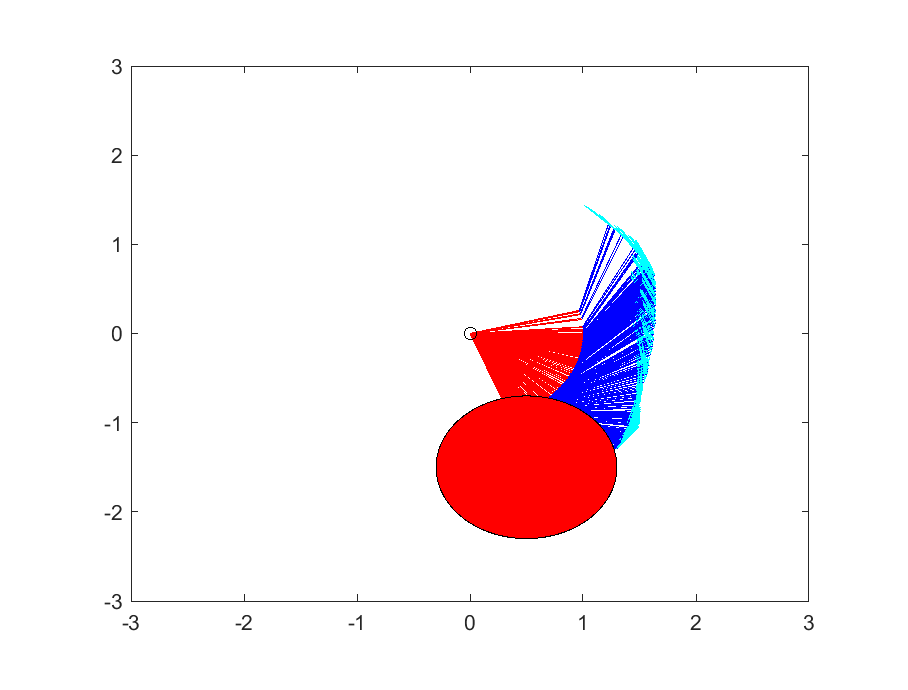
\includegraphics[width=0.35\textwidth]{qdp1.eps}
	\caption{Trajectória com controlo aplicado, em que $K_q=0$ e $q_{dp}=\left[0~0~0\right]^T $.}
\label{qdp1}
\end{figure}
O robô mantém a postura deslocando-se para a posição desejada,  entretanto, desconsiderando a região vital, sendo esta uma característica não pretendida, uma vez que, em casos clínicos, implicaria numa situação de risco e até mesmo fatal para o paciente.

\section{Criativo}
 Nesta parte do trabalho, decidimos utilizar o controlo efectuado na secção (2.8) para implementar uma simulação de extracção de medula óssea, seja para a finalidade de exame ou transplante.
Para realizar esta tarefa, primeiramente, é preciso considerar a anatomia do osso, representado na figura \ref{figosso}.
 \begin{figure}[H]
	\centering
	\includegraphics[width=0.35\textwidth]{osso.jpg}
	\caption{Componentes do tecido ósseo \cite{bone}.}
  \label{figosso}
\end{figure}
 O osso é constituído por diversas estruturas, como células e tecidos, dentre as quais iremos considerar o osso compacto, seguido por um osso esponjoso e por fim a medula óssea.
 Para a implementação do osso esponjoso, consideramos que o robô, após atravessar o osso compacto irá deparar-se com uma rigidez inferior correspondente ao osso esponjoso.
 Portanto, fez-se necessário implementar valores para traduzir esta menor rigidez, com:
\begin{equation}
    K_{e_{Mole}}=[100~0; 0~0]
\end{equation}

\\ 
A medula, por ser líquida, apresenta uma rigidez extremamente pequena, e portanto, para esta implementação foi desconsiderada.

\\
Para além disso, após o robô alcançar a medula, e realizar uma possível raspagem ou aspiração, é necessário que este retorne até ao ponto de partida.
Para isto, acrescentou-se na implementação no Simulink a função \textit{turnfun}, a qual tem por finalidade indicar ao robô quando deve retornar.
\begin{figure}[H]
	\centering
	\includegraphics[width=0.5\textwidth]{simulink.png}
	\caption{Implementação Simulink}
\label{simulink}
\end{figure}
\\
Quando for necessário o regresso do robô, as forças do robô e do médico tornam-se negativas, e ao chegar no ponto desejado de paragem, estas são ajustadas de forma a que o robô não se mova mais. 

\\
A força de amortecimento também foi ajustada conforme necessário, para que o robô não apresente oscilações que podem ocasionar risco ao paciente.
Este robô foi, assim, desenhado para que pudesse alterar os valores da matriz $K_p$ e da matriz $K_D$ durante a execução da sua tarefa, de forma a poder executar, por exemplo, uma extracção de medula em segurança. 

\begin{figure}[H]
	\centering
	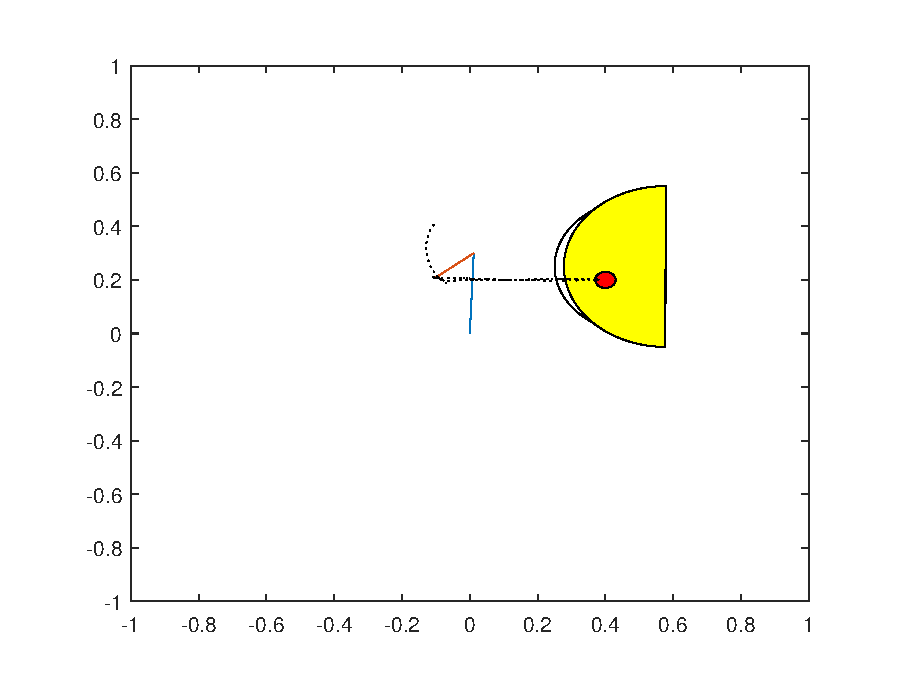
\includegraphics[width=0.4\textwidth]{medula.eps}
	\caption{Trajectória para procedimentos realizados na medula óssea.}
\label{medula}
\end{figure}

 Consideramos também que, caso o médico realize uma força muito discrepante ou desnecessária, esta anular-se-à, anulando também todos os componentes da matriz $K_D$.


\begin{thebibliography}{9}
\bibitem{project}
Cortesão, R. (2019). Medical Robotics Project - 2019/2020. Control and Trajectory Design for Bone Surgeries.

\bibitem{Cortesão}
Cortesão, R. (2019). Medical Robotics Course.

\bibitem{Spong}
Spong, M., Vidyasagar, M. and Hutchinson, S. (2004). Robot dynamics and control. 2nd ed. p.Chapter 9.

\bibitem{Sleewee}
Sleewee. (2019). Long Bone Anatomy: Structure and Parts of Long Bones. [online] Available at: \url{https://www.sleewee.com/parts-of-long-bones} [Accessed 2019].

\bibitem{bone}
Narayanahealth.org. (2020). Bone Marrow Transplant: Disease, Procedure & Cost | Narayana Health. [online] Available at: https://www.narayanahealth.org/bone-marrow-transplant/.

\bibitem{Netter}
Netter. (2014). Atlas of Human Anatomy, Sixth Edition. Elsevier.


\end{thebibliography}


\end{document}